\documentclass{article}
\usepackage{graphicx}
\usepackage{caption}
\usepackage{subcaption}
\usepackage{float}
\usepackage{chngpage}

\begin{document}

\title{Estimating A Modified Ball-and-sticks Diffusion Model with Expectation Maximization and Rician Likelihood}
\author{Xinghua Zhu}

\maketitle

\begin{abstract}
  This is a summary of the modified ball-and sticks model estimation experiments.
\end{abstract}

%\section{Introduction}
%Here is the text of your introduction.


\section{Estimating weights V.S. diffusivities}
\subsection{Synthesized data}

In the following figures series of DW data are synthesized with different diffusivities and weights.
\subsubsection{Multiplicative Ball-And-Sticks Model}
\begin{figure}[H]
  \begin{adjustwidth}{-\oddsidemargin}{-\rightmargin}
    \begin{subfigure}{0.8\paperwidth}
      \begin{subfigure}{0.3\textwidth}
        \centering
        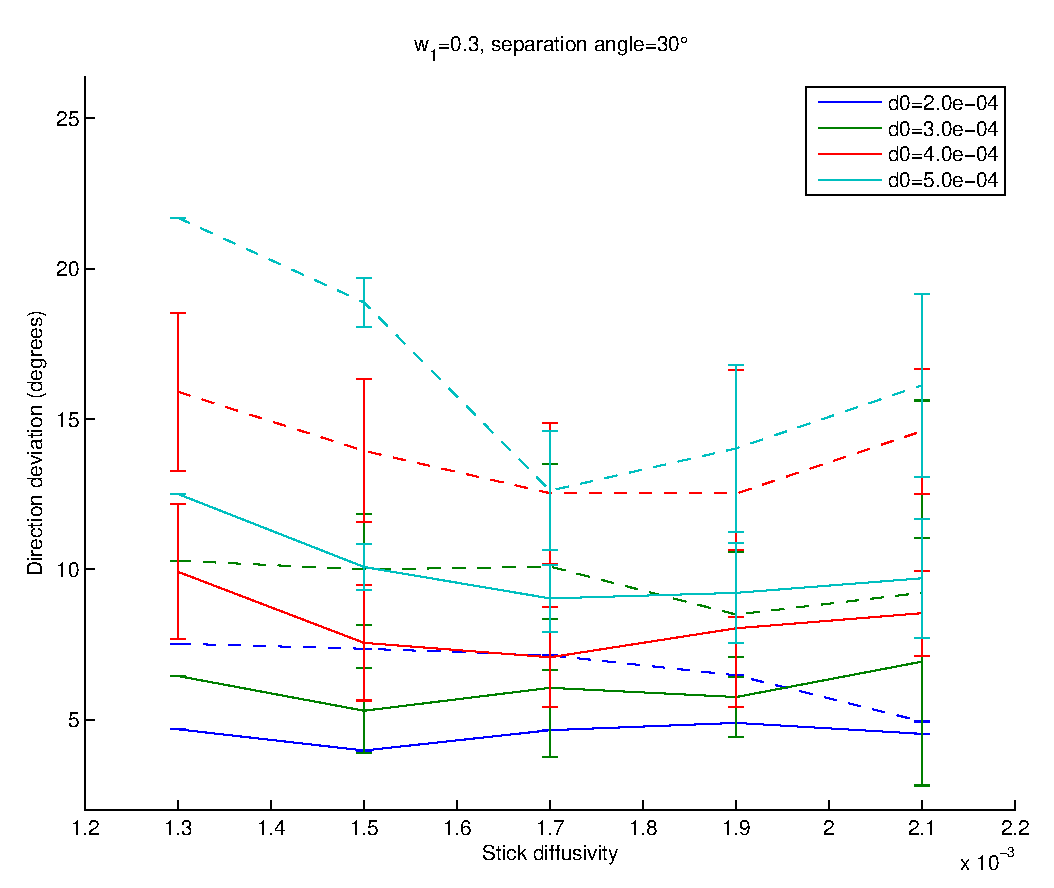
\includegraphics[width=\textwidth]{figures/synth_modbas_weights__snr=20__w1=3__angle=30.eps}
      \end{subfigure}
      ~
      \begin{subfigure}{0.3\textwidth}
        \centering
        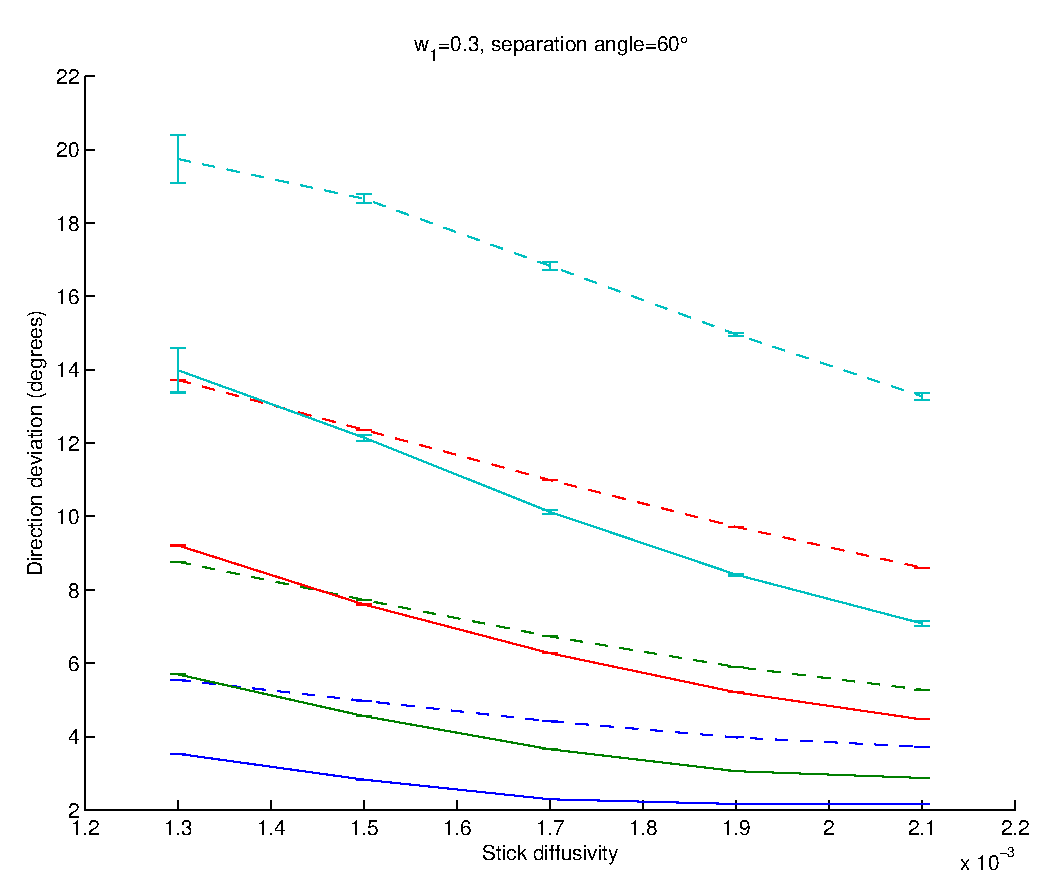
\includegraphics[width=\textwidth]{figures/synth_modbas_weights__snr=20__w1=3__angle=60.eps}
      \end{subfigure}
      ~
      \begin{subfigure}{0.3\textwidth}
        \centering
        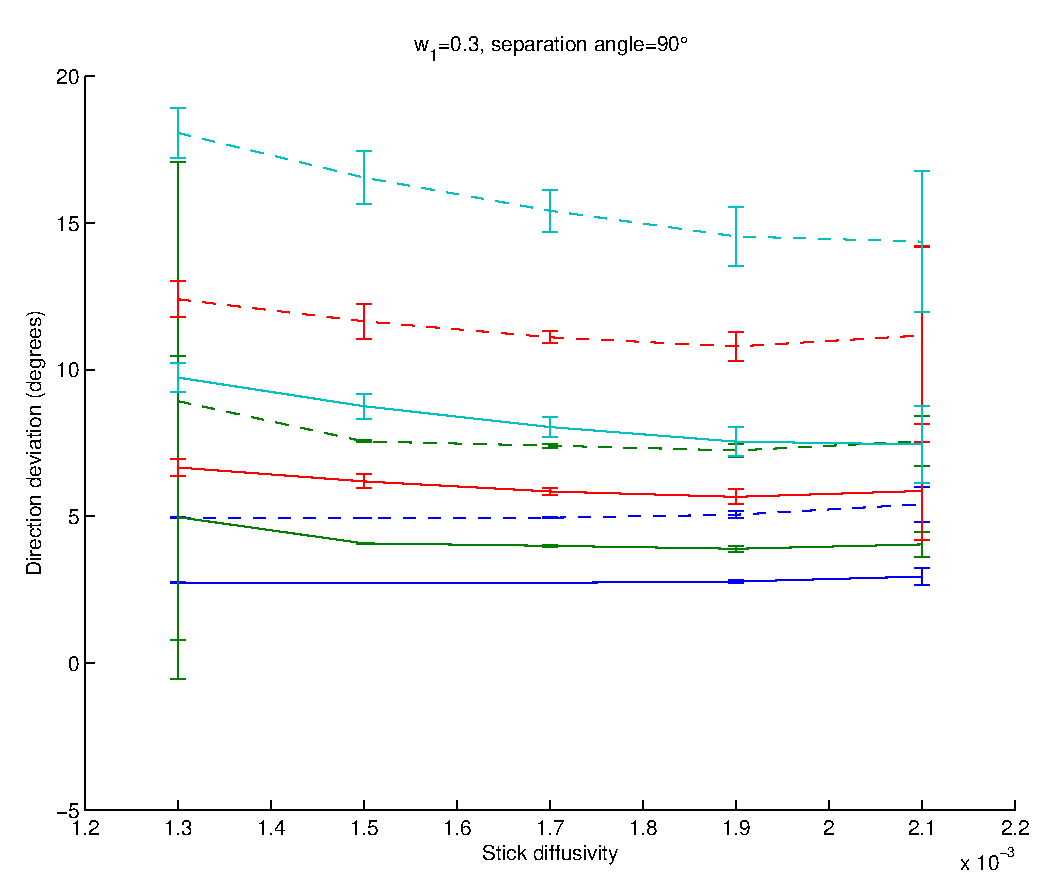
\includegraphics[width=\textwidth]{figures/synth_modbas_weights__snr=20__w1=3__angle=90.eps}
      \end{subfigure}
    \end{subfigure}
    
    \begin{subfigure}{0.8\paperwidth}
      \begin{subfigure}{0.3\textwidth}
        \centering
        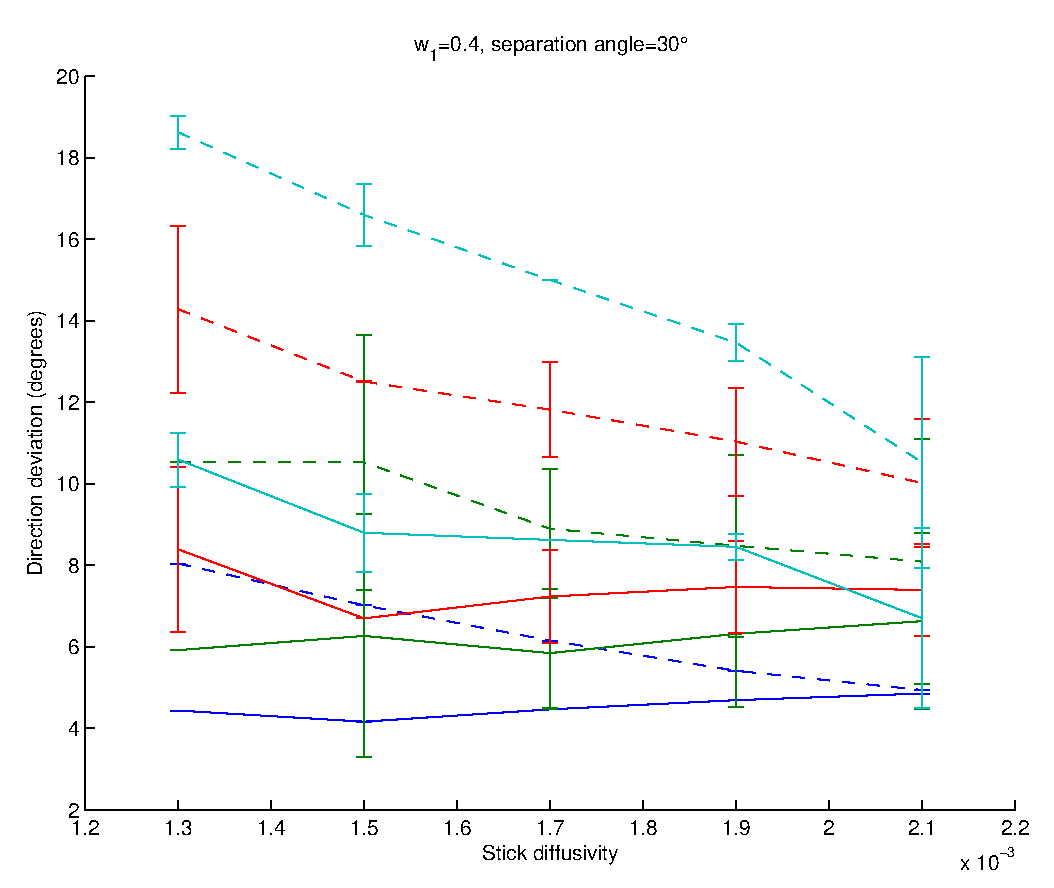
\includegraphics[width=\textwidth]{figures/synth_modbas_weights__snr=20__w1=4__angle=30.eps}
      \end{subfigure}
      ~
      \begin{subfigure}{0.3\textwidth}
        \centering
        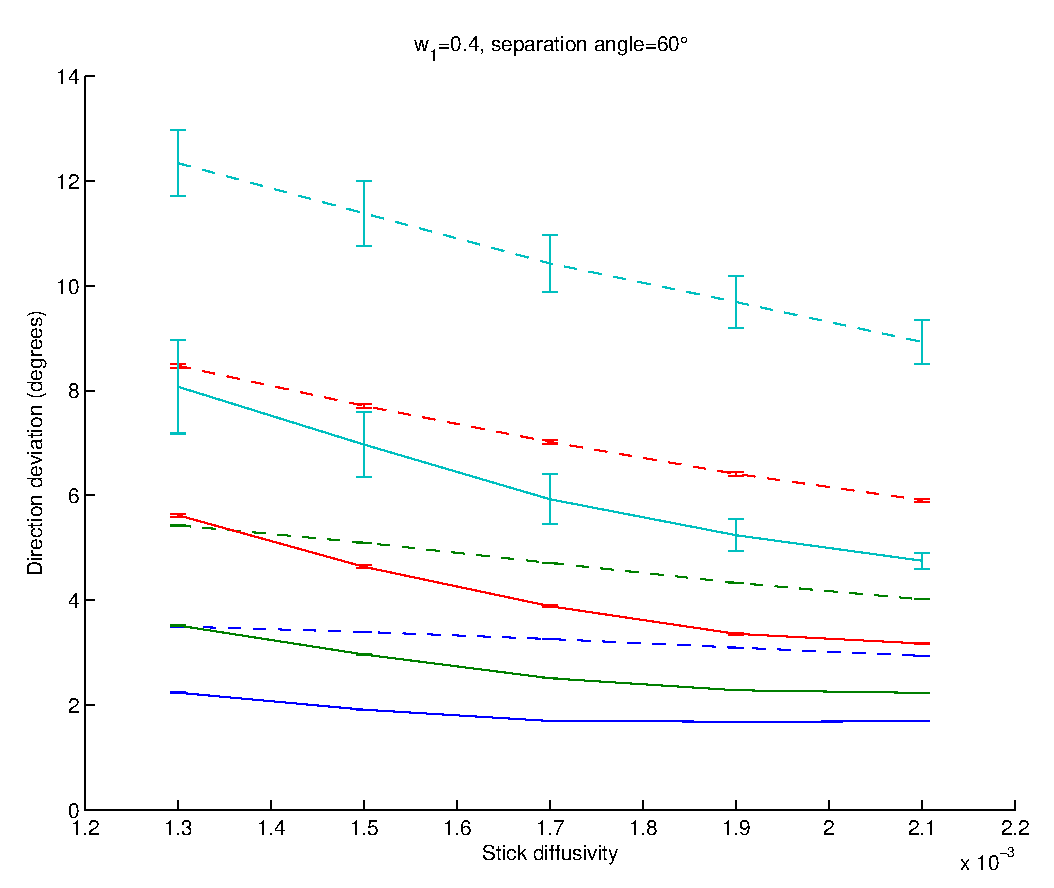
\includegraphics[width=\textwidth]{figures/synth_modbas_weights__snr=20__w1=4__angle=60.eps}
      \end{subfigure}
      ~
      \begin{subfigure}{0.3\textwidth}
        \centering
        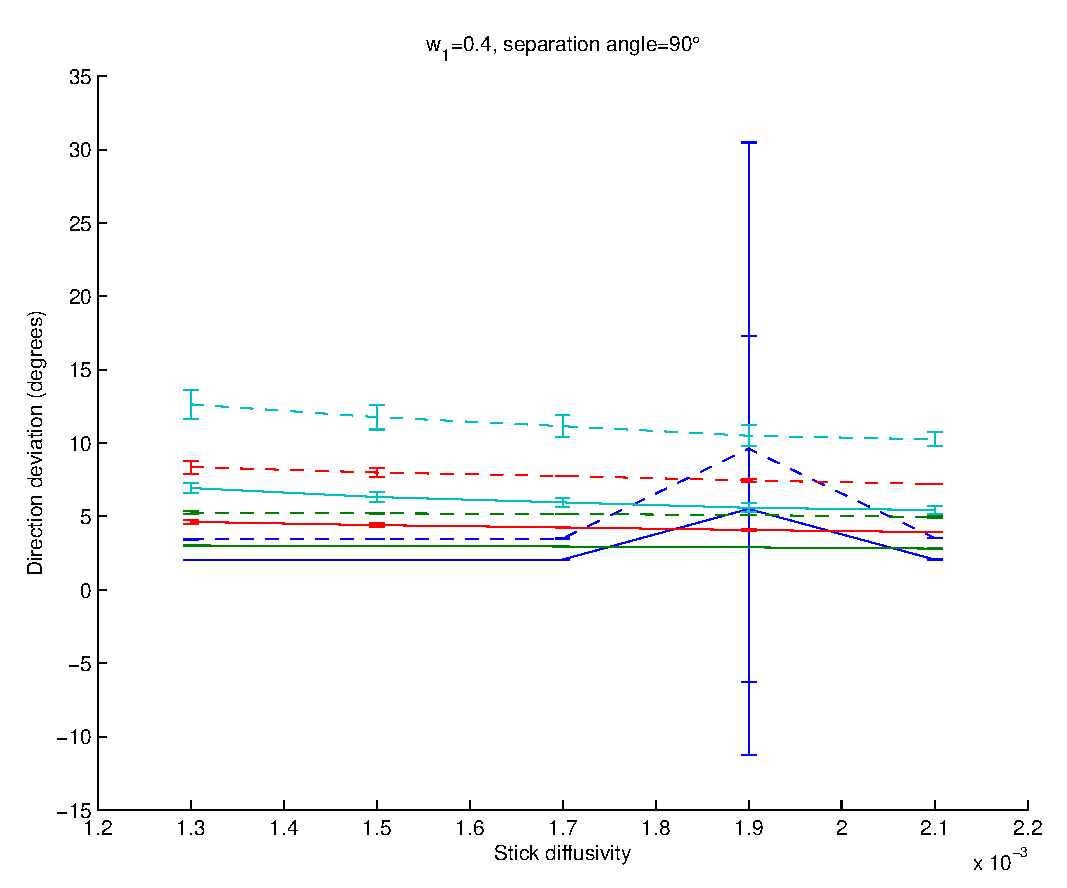
\includegraphics[width=\textwidth]{figures/synth_modbas_weights__snr=20__w1=4__angle=90.eps}
      \end{subfigure}
    \end{subfigure}
    \begin{subfigure}{0.8\paperwidth}
      \begin{subfigure}{0.3\textwidth}
        \centering
        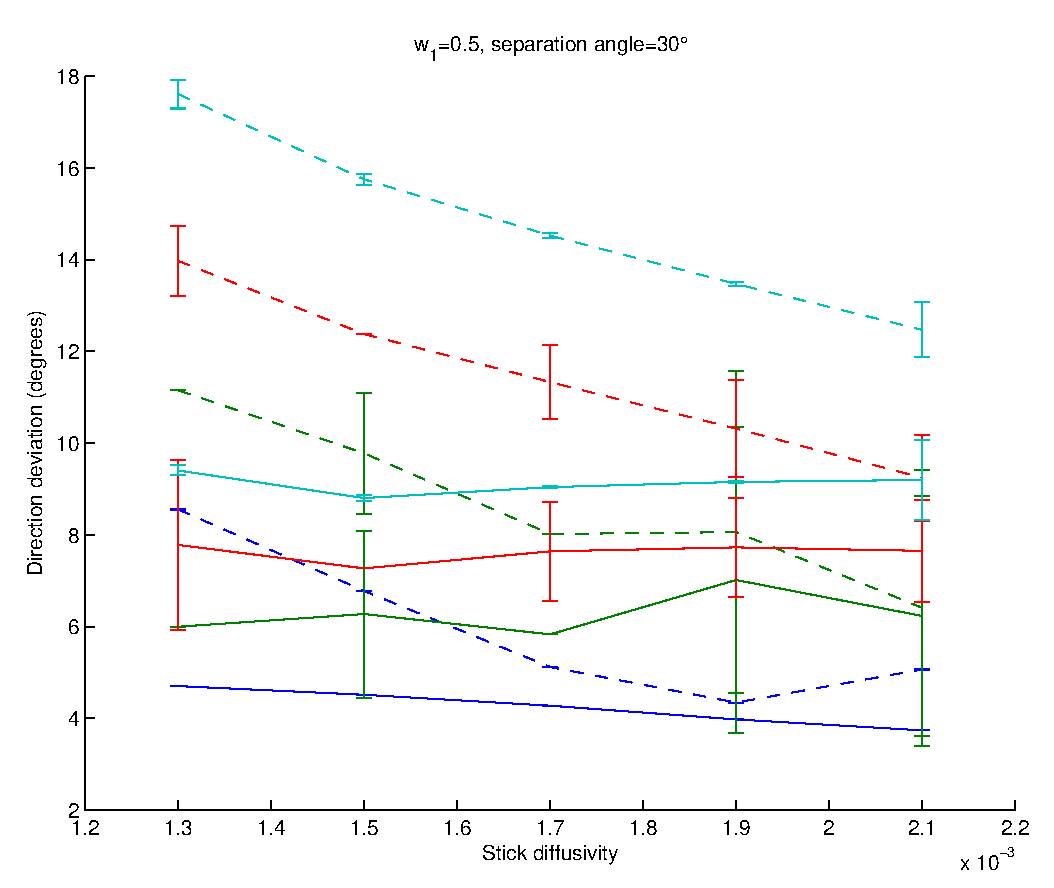
\includegraphics[width=\textwidth]{figures/synth_modbas_weights__snr=20__w1=5__angle=30.eps}
      \end{subfigure}
      ~
      \begin{subfigure}{0.3\textwidth}
        \centering
        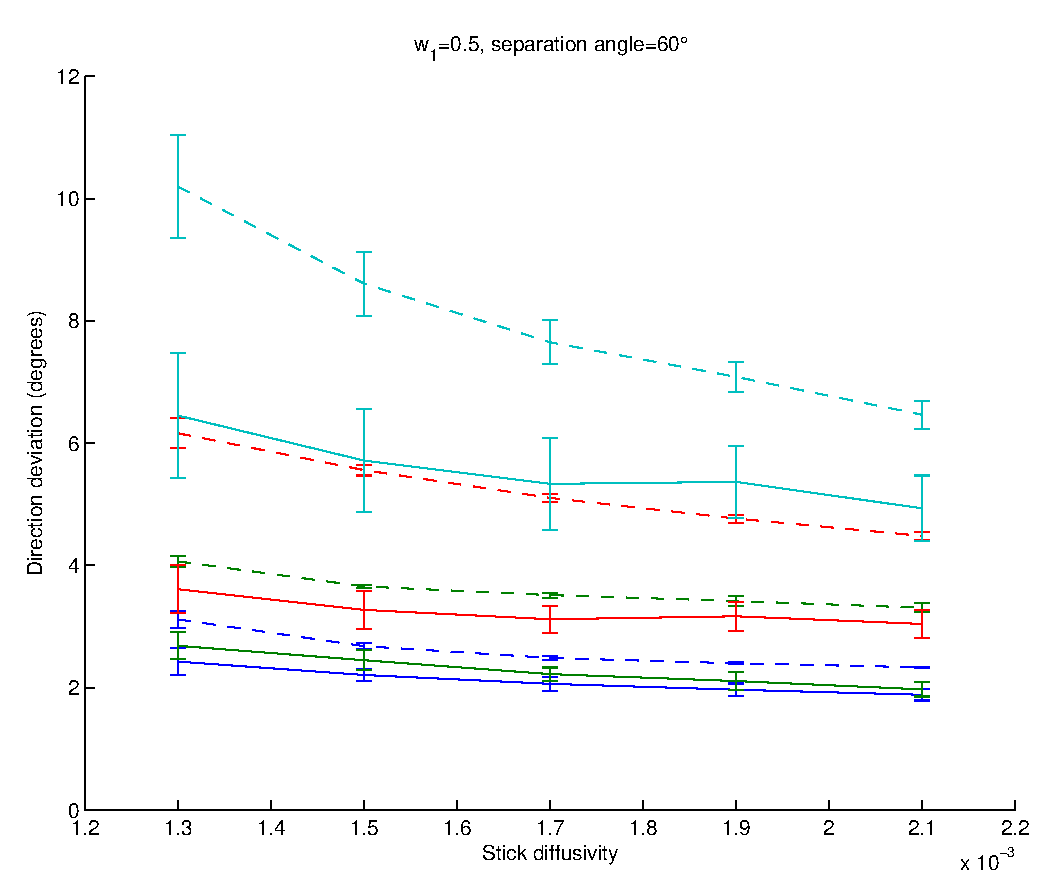
\includegraphics[width=\textwidth]{figures/synth_modbas_weights__snr=20__w1=5__angle=60.eps}
      \end{subfigure}
      ~
      \begin{subfigure}{0.3\textwidth}
        \centering
        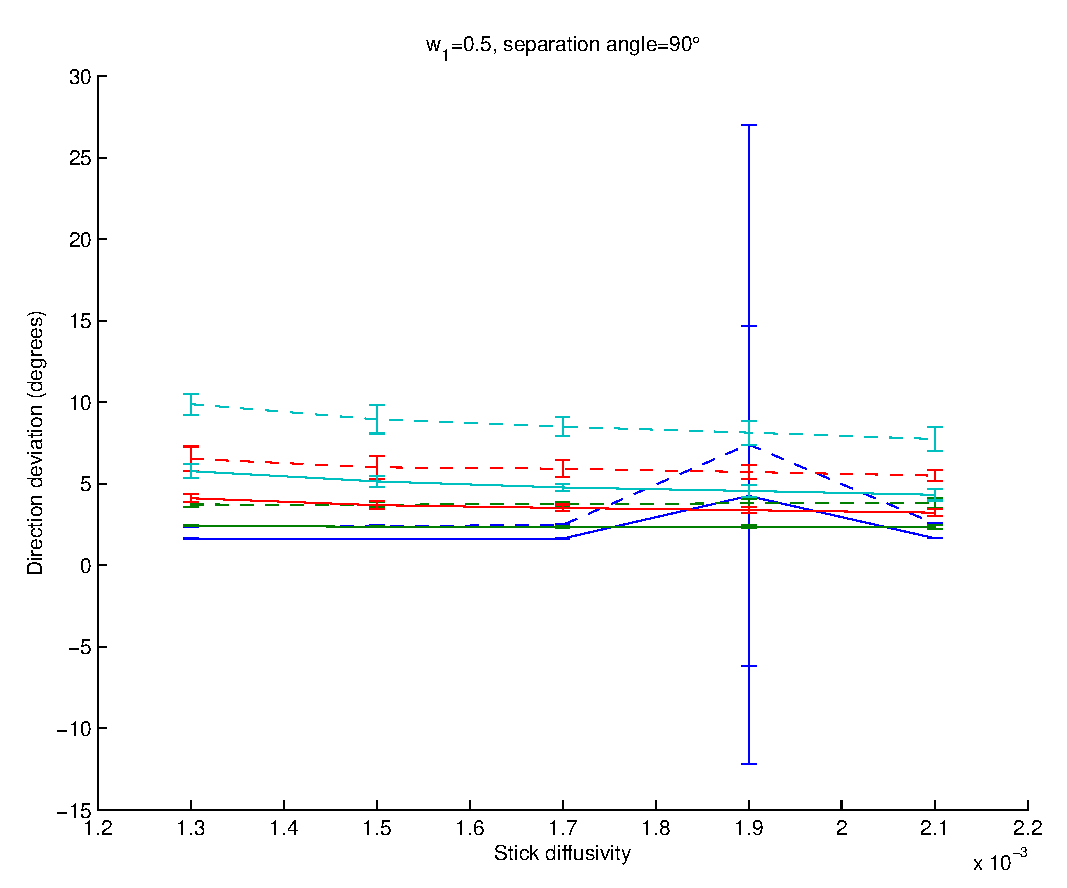
\includegraphics[width=\textwidth]{figures/synth_modbas_weights__snr=20__w1=5__angle=90.eps}
      \end{subfigure}
    \end{subfigure}
  \end{adjustwidth}
  
  \caption{Estimation results with weight and ball-diffusivity estimation. Stick diffusivities are fixed at $1.7\times 10^{-3}$. From top to bottom: synthesized weights are (0.3, 0.7), (0.4, 0.6), (0.5, 0.5) respectively. From left to right: separation angles are 30, 60 and 90 degrees, respectively. Simulated SNR is 20.}
\end{figure}

\begin{figure}[H]
  \begin{adjustwidth}{-\oddsidemargin}{-\rightmargin}
    \begin{subfigure}{0.8\paperwidth}
      \begin{subfigure}{0.3\textwidth}
        \centering
        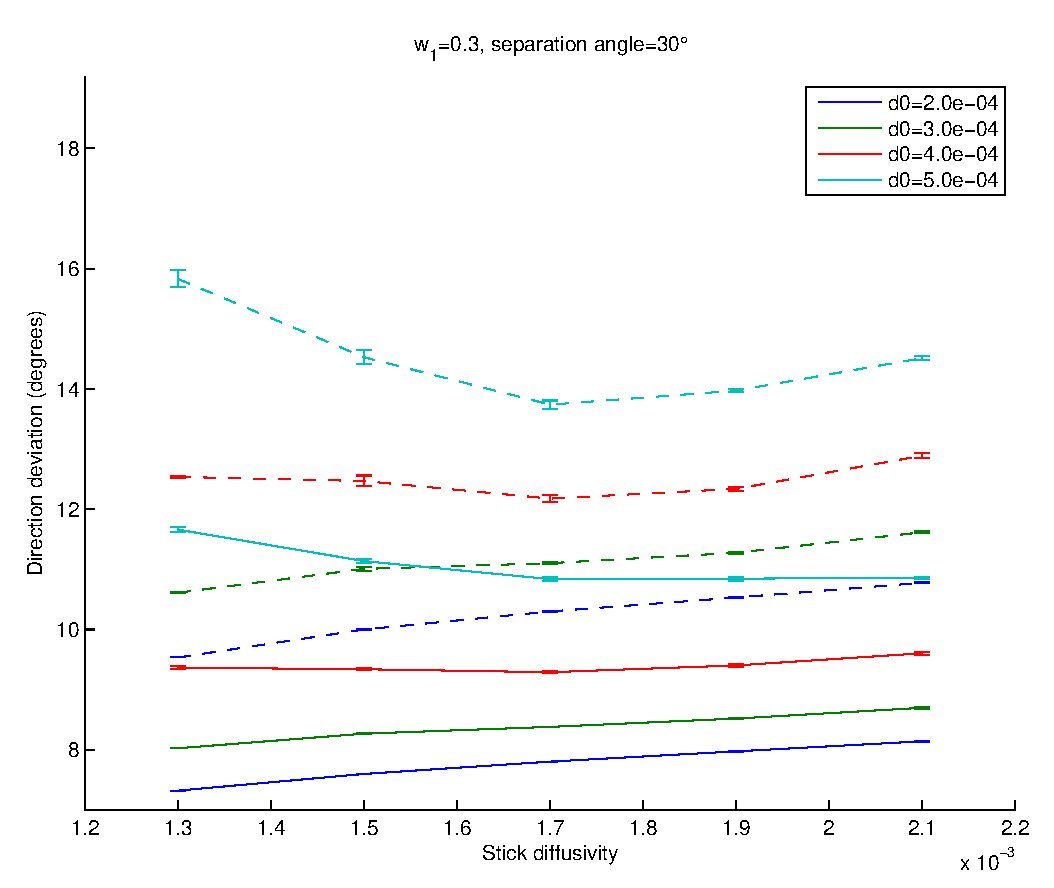
\includegraphics[width=\textwidth]{figures/synth_modbas_diffus__snr=20__w1=3__angle=30.eps}
      \end{subfigure}
      ~
      \begin{subfigure}{0.3\textwidth}
        \centering
        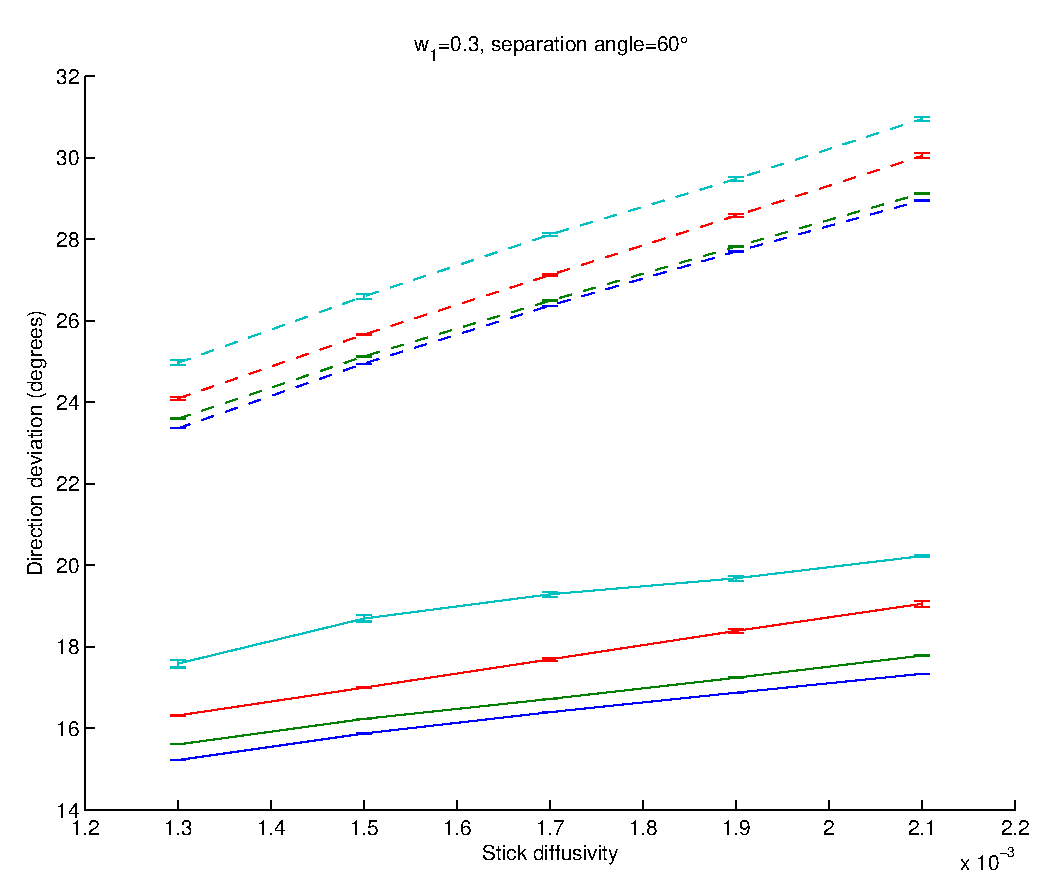
\includegraphics[width=\textwidth]{figures/synth_modbas_diffus__snr=20__w1=3__angle=60.eps}
      \end{subfigure}
      ~
      \begin{subfigure}{0.3\textwidth}
        \centering
        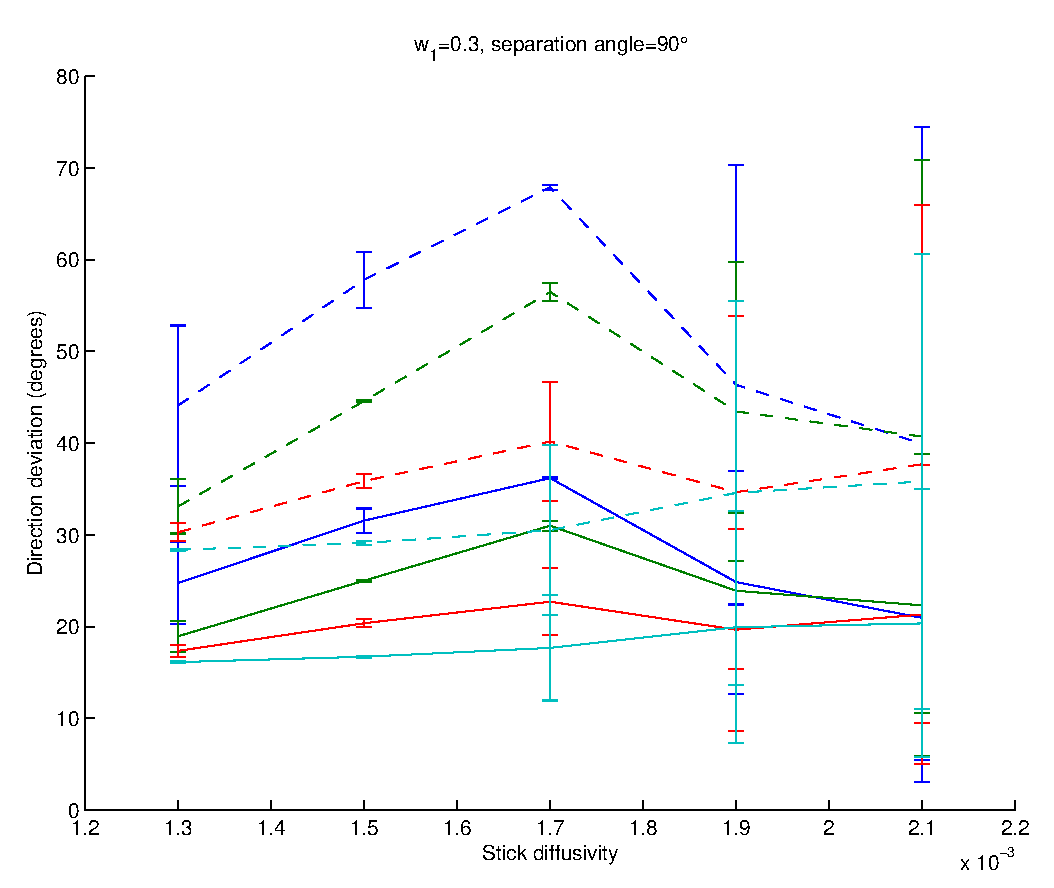
\includegraphics[width=\textwidth]{figures/synth_modbas_diffus__snr=20__w1=3__angle=90.eps}
      \end{subfigure}
    \end{subfigure}
    
    \begin{subfigure}{0.8\paperwidth}
      \begin{subfigure}{0.3\textwidth}
        \centering
        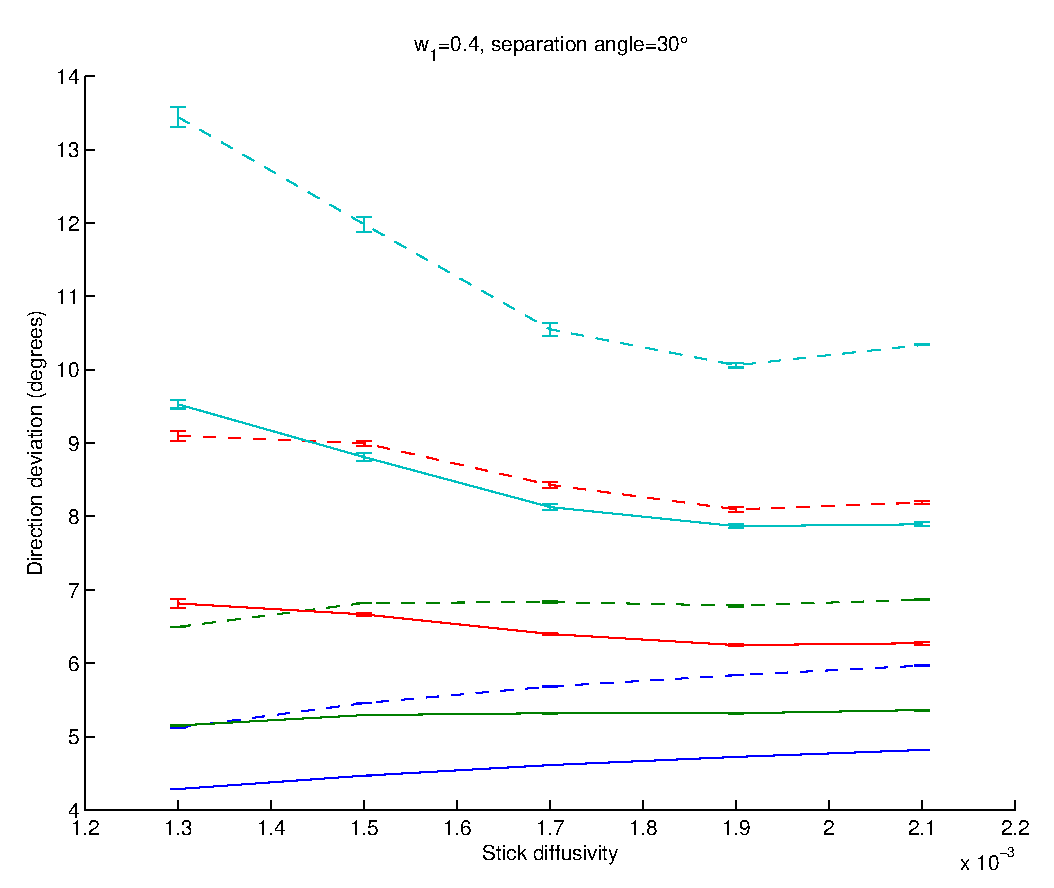
\includegraphics[width=\textwidth]{figures/synth_modbas_diffus__snr=20__w1=4__angle=30.eps}
      \end{subfigure}
      ~
      \begin{subfigure}{0.3\textwidth}
        \centering
        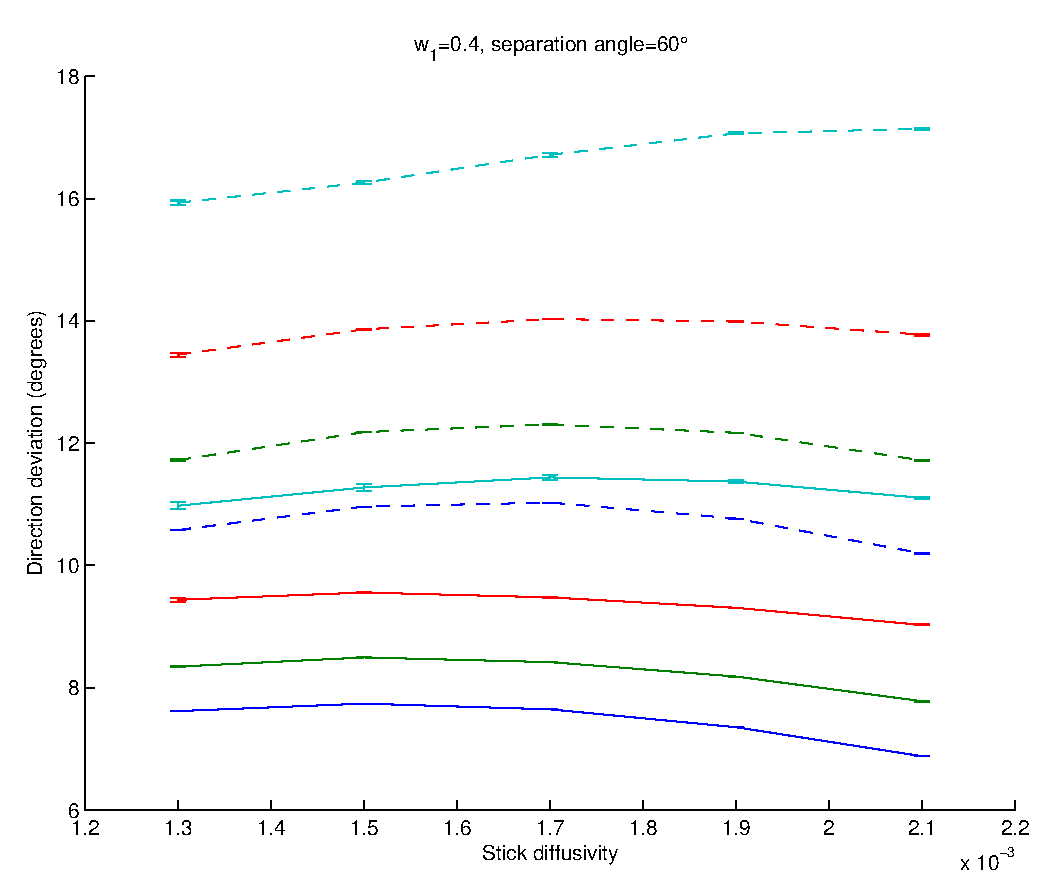
\includegraphics[width=\textwidth]{figures/synth_modbas_diffus__snr=20__w1=4__angle=60.eps}
      \end{subfigure}
      ~
      \begin{subfigure}{0.3\textwidth}
        \centering
        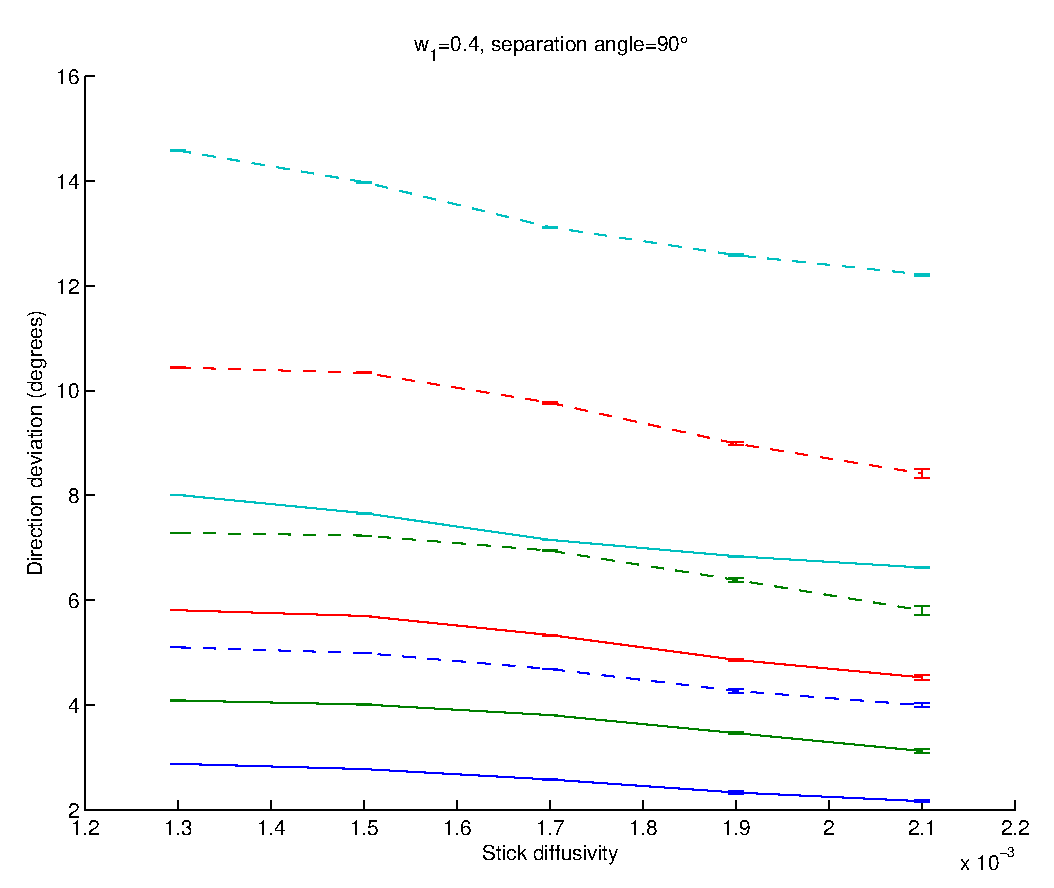
\includegraphics[width=\textwidth]{figures/synth_modbas_diffus__snr=20__w1=4__angle=90.eps}
      \end{subfigure}
    \end{subfigure}
    \begin{subfigure}{0.8\paperwidth}
      \begin{subfigure}{0.3\textwidth}
        \centering
        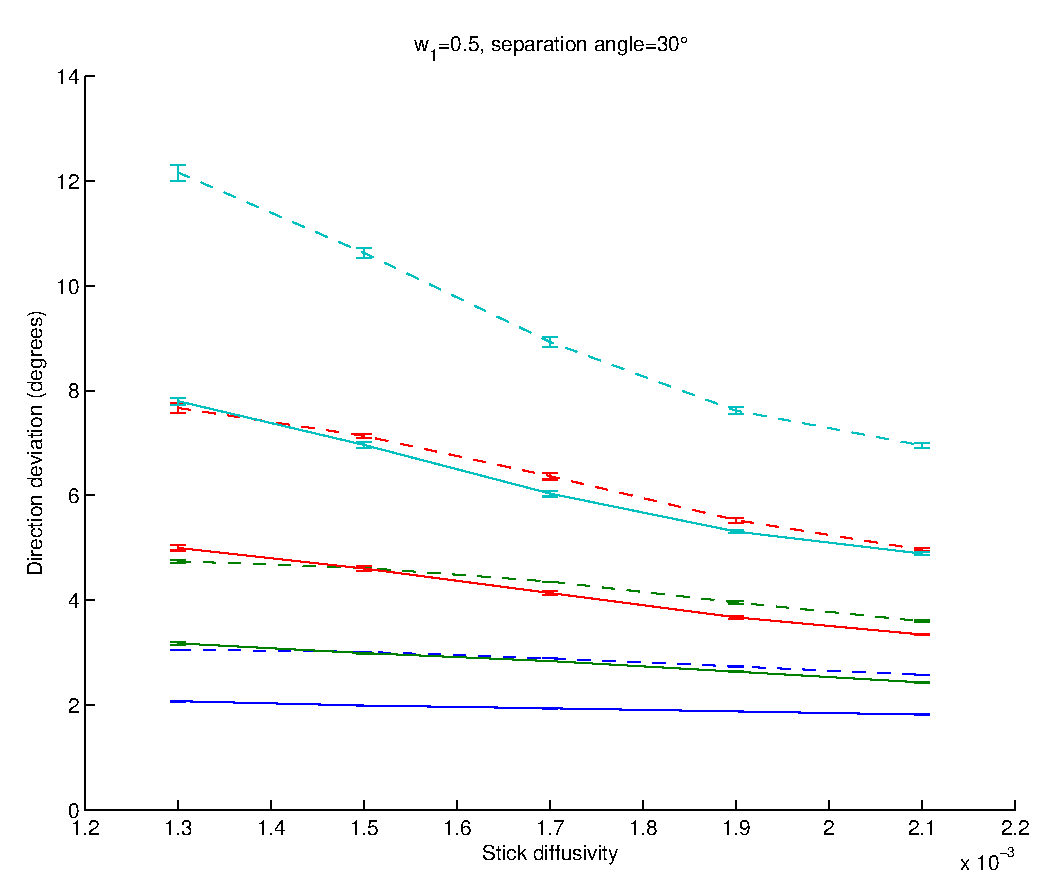
\includegraphics[width=\textwidth]{figures/synth_modbas_diffus__snr=20__w1=5__angle=30.eps}
      \end{subfigure}
      ~
      \begin{subfigure}{0.3\textwidth}
        \centering
        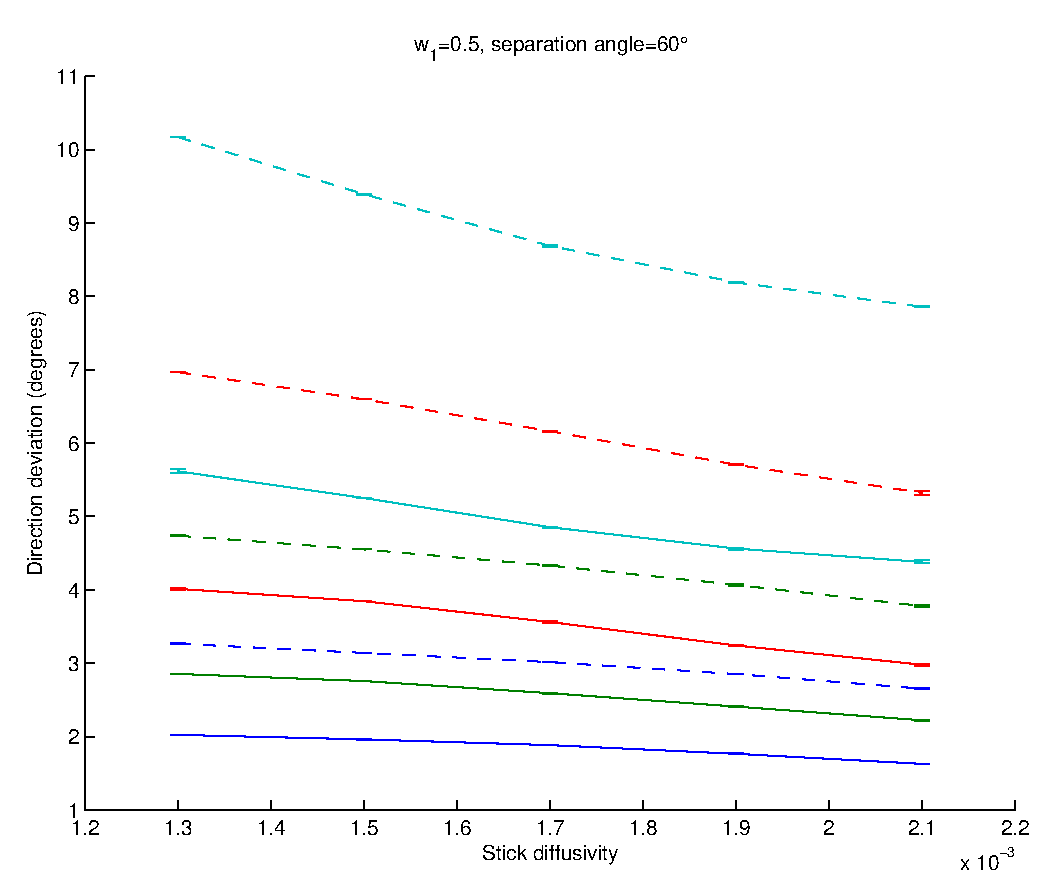
\includegraphics[width=\textwidth]{figures/synth_modbas_diffus__snr=20__w1=5__angle=60.eps}
      \end{subfigure}
      ~
      \begin{subfigure}{0.3\textwidth}
        \centering
        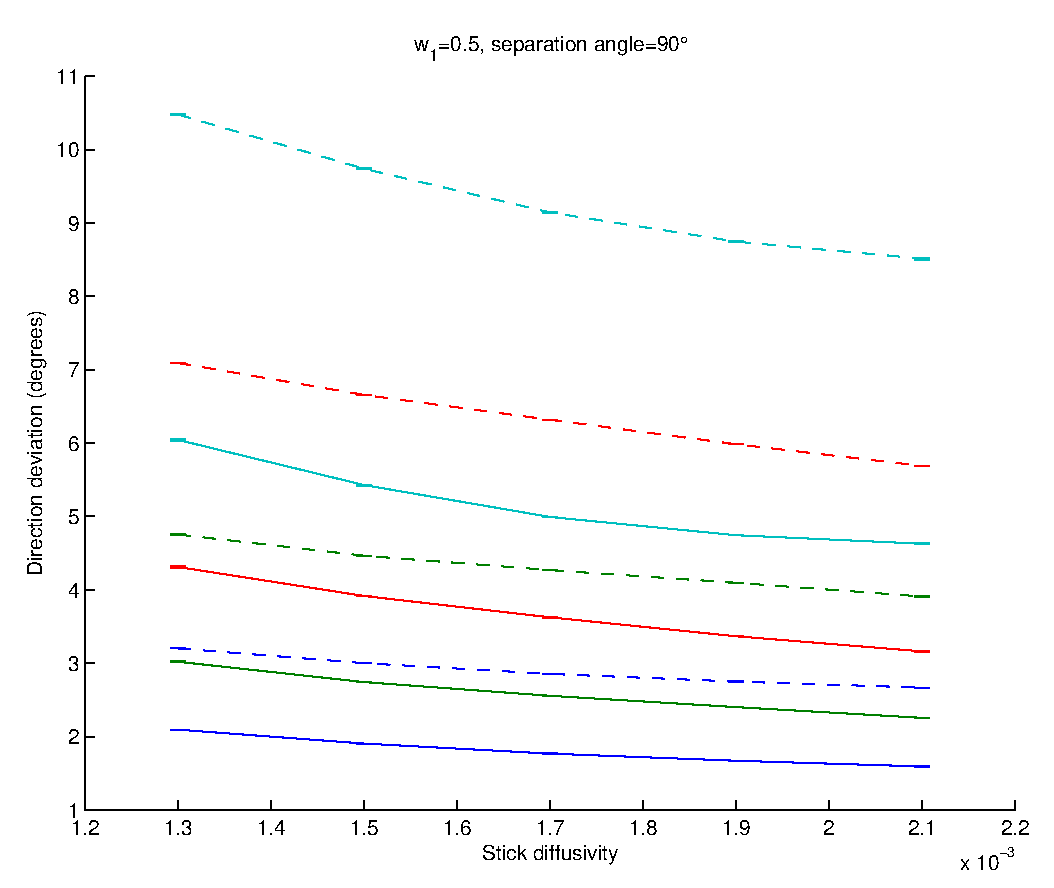
\includegraphics[width=\textwidth]{figures/synth_modbas_diffus__snr=20__w1=5__angle=90.eps}
      \end{subfigure}
    \end{subfigure}
  \end{adjustwidth}
  
  \caption{Estimation results with diffusivity estimation. Weights are fixed at (0.5, 0.5). From top to bottom: synthesized weights are (0.3, 0.7), (0.4, 0.6), (0.5, 0.5) respectively. From left to right: separation angles are 30, 60 and 90 degrees, respectively. Simulated SNR is 20.}
\end{figure}

\begin{figure}[H]
  \begin{adjustwidth}{-\oddsidemargin}{-\rightmargin}
    \begin{subfigure}{0.8\paperwidth}
      \begin{subfigure}{0.3\textwidth}
        \centering
        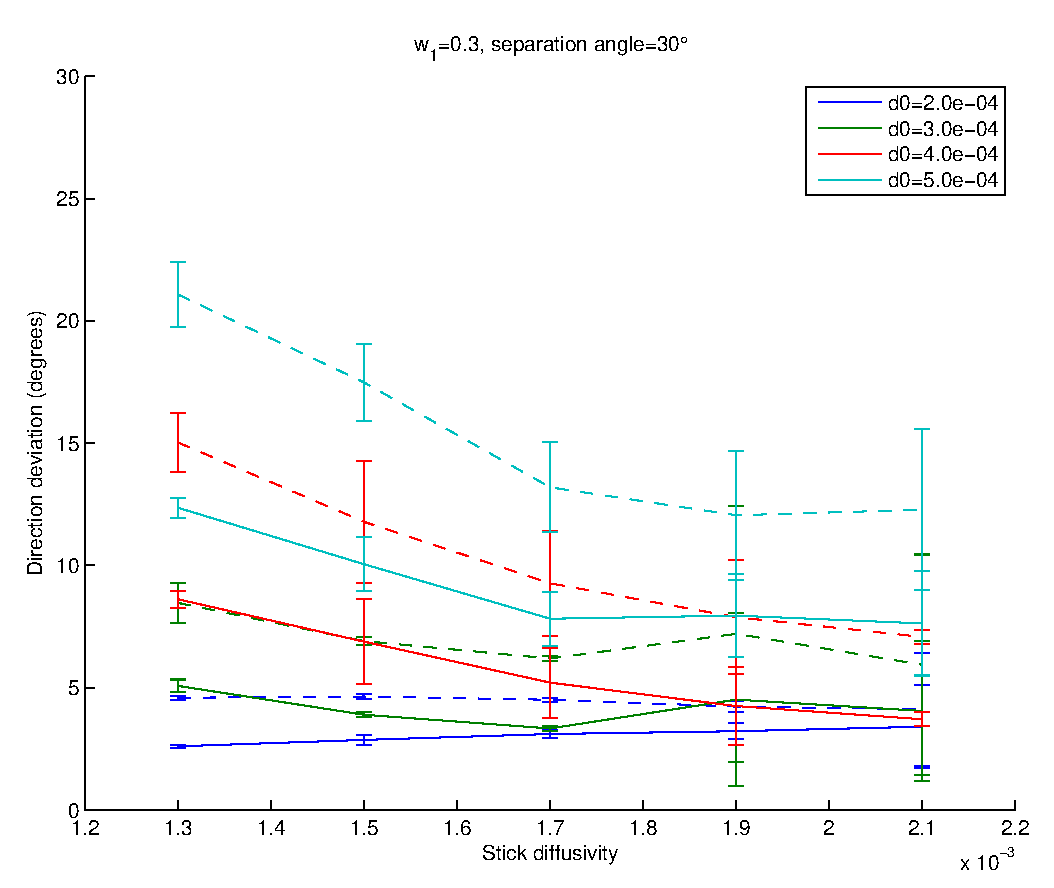
\includegraphics[width=\textwidth]{figures/synth_modbas_weights_diffus__snr=20__w1=3__angle=30.eps}
      \end{subfigure}
      ~
      \begin{subfigure}{0.3\textwidth}
        \centering
        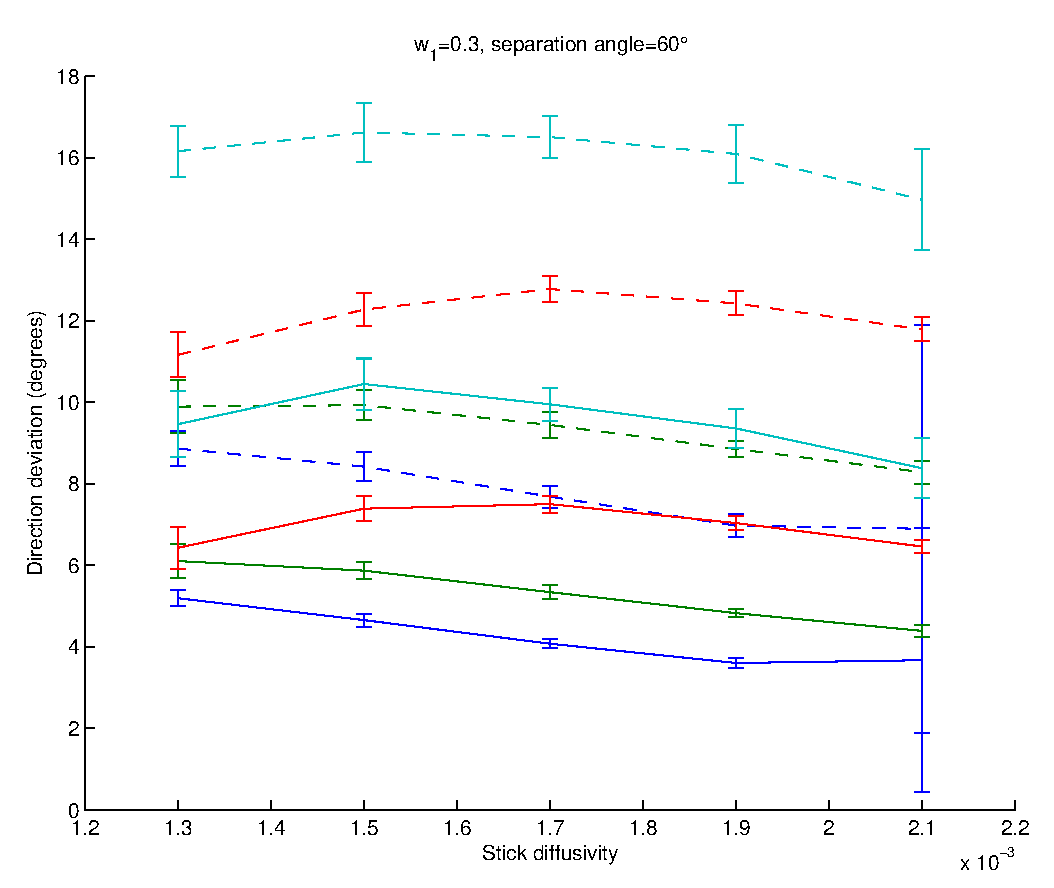
\includegraphics[width=\textwidth]{figures/synth_modbas_weights_diffus__snr=20__w1=3__angle=60.eps}
      \end{subfigure}
      ~
      \begin{subfigure}{0.3\textwidth}
        \centering
        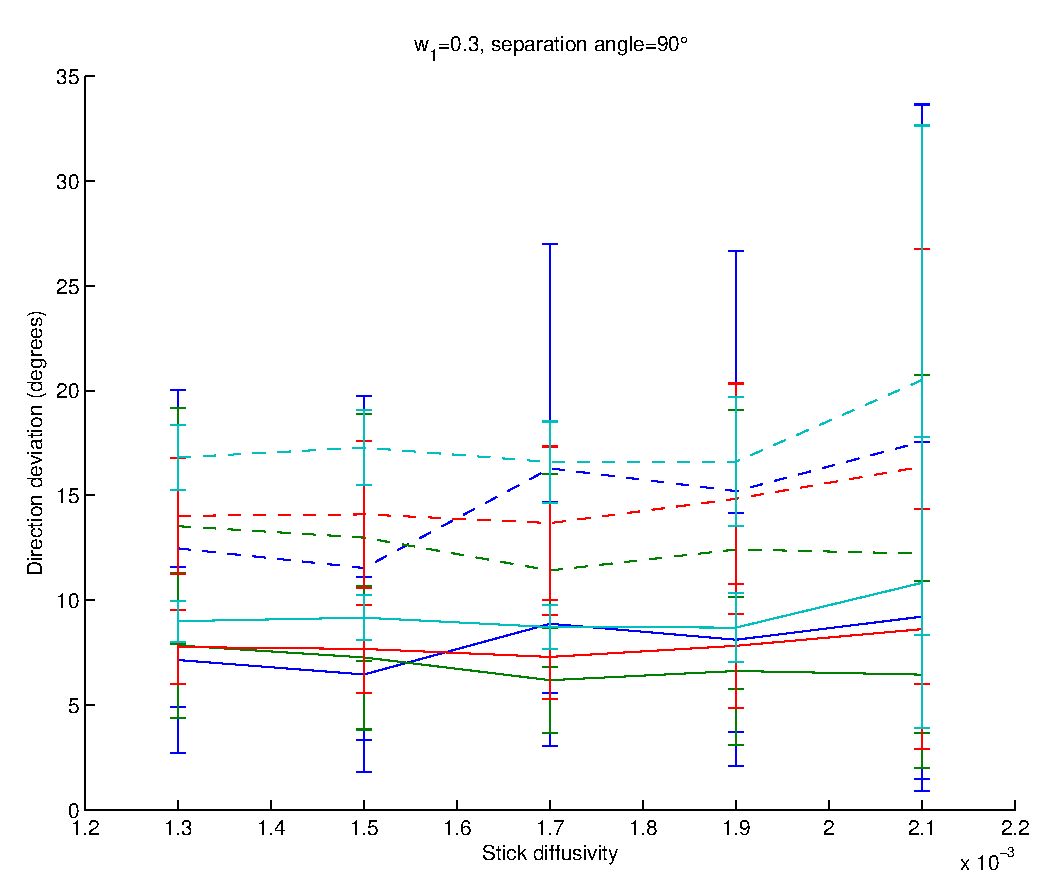
\includegraphics[width=\textwidth]{figures/synth_modbas_weights_diffus__snr=20__w1=3__angle=90.eps}
      \end{subfigure}
  \end{subfigure}

  \begin{subfigure}{0.8\paperwidth}
    \begin{subfigure}{0.3\textwidth}
      \centering
      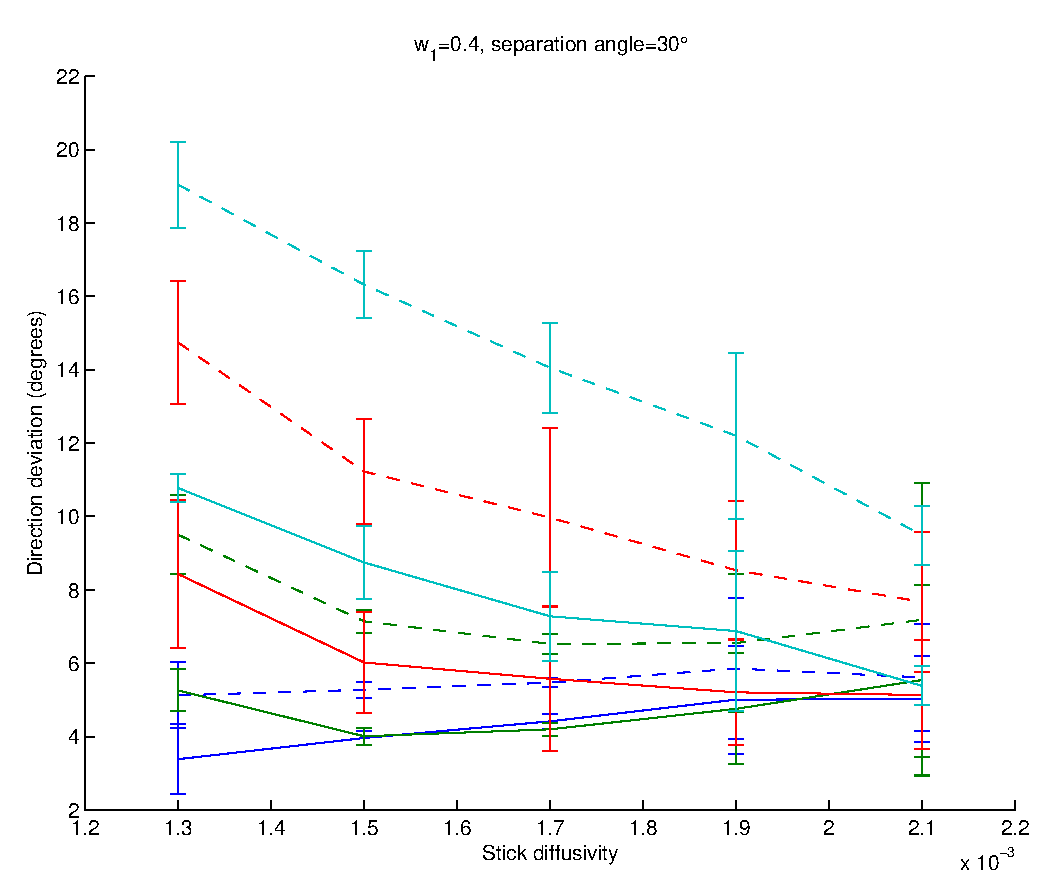
\includegraphics[width=\textwidth]{figures/synth_modbas_weights_diffus__snr=20__w1=4__angle=30.eps}
    \end{subfigure}
      ~
      \begin{subfigure}{0.3\textwidth}
        \centering
        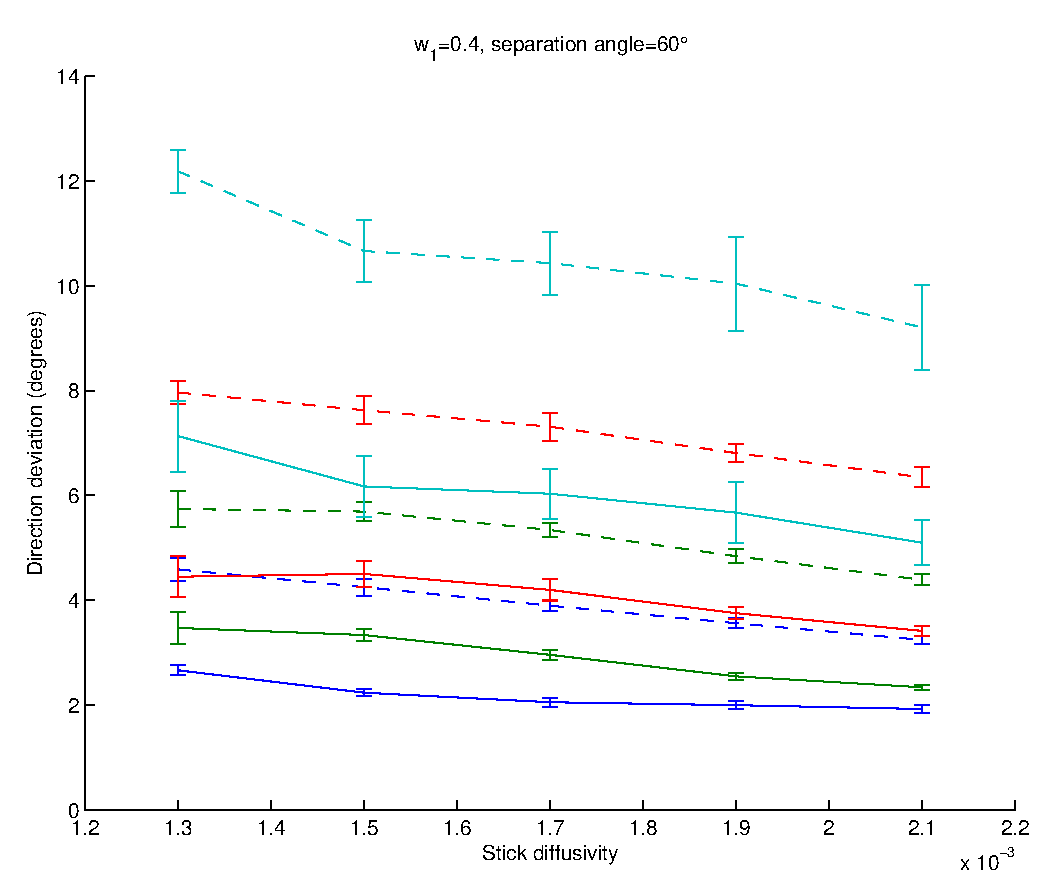
\includegraphics[width=\textwidth]{figures/synth_modbas_weights_diffus__snr=20__w1=4__angle=60.eps}
      \end{subfigure}
      ~
      \begin{subfigure}{0.3\textwidth}
        \centering
        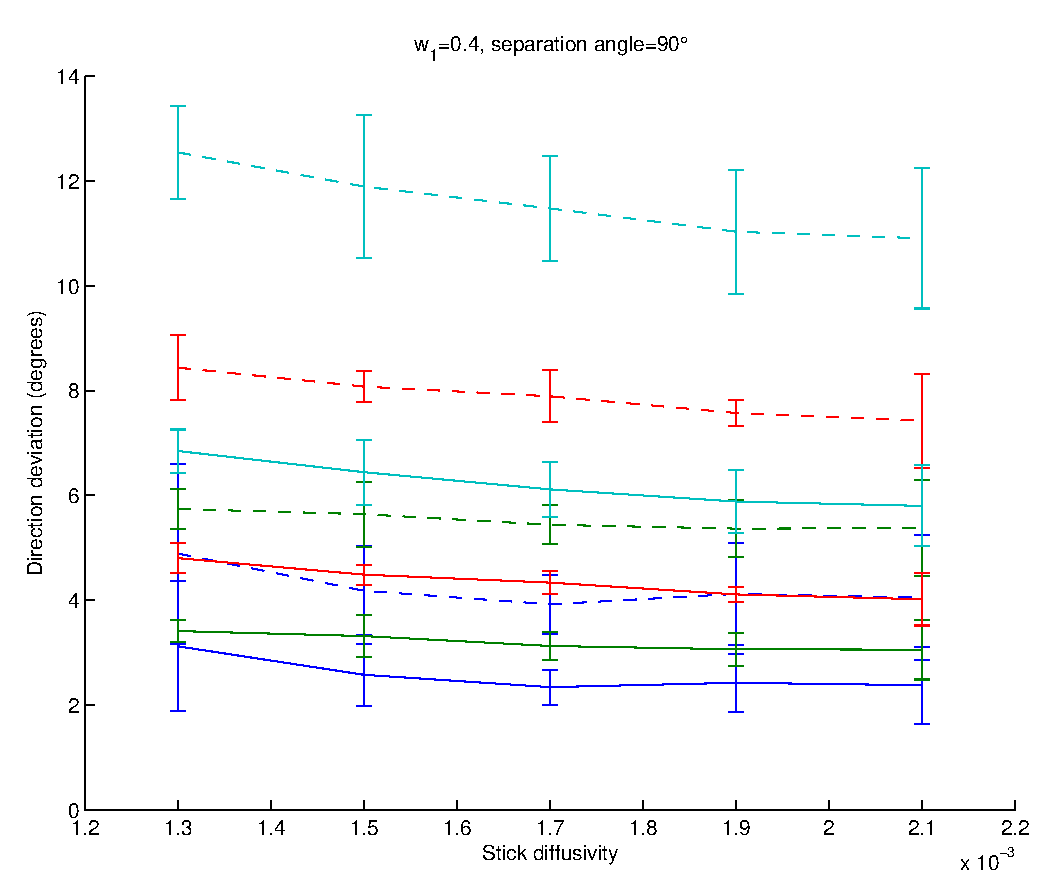
\includegraphics[width=\textwidth]{figures/synth_modbas_weights_diffus__snr=20__w1=4__angle=90.eps}
      \end{subfigure}
  \end{subfigure}
  \begin{subfigure}{0.8\paperwidth}
      \begin{subfigure}{0.3\textwidth}
        \centering
        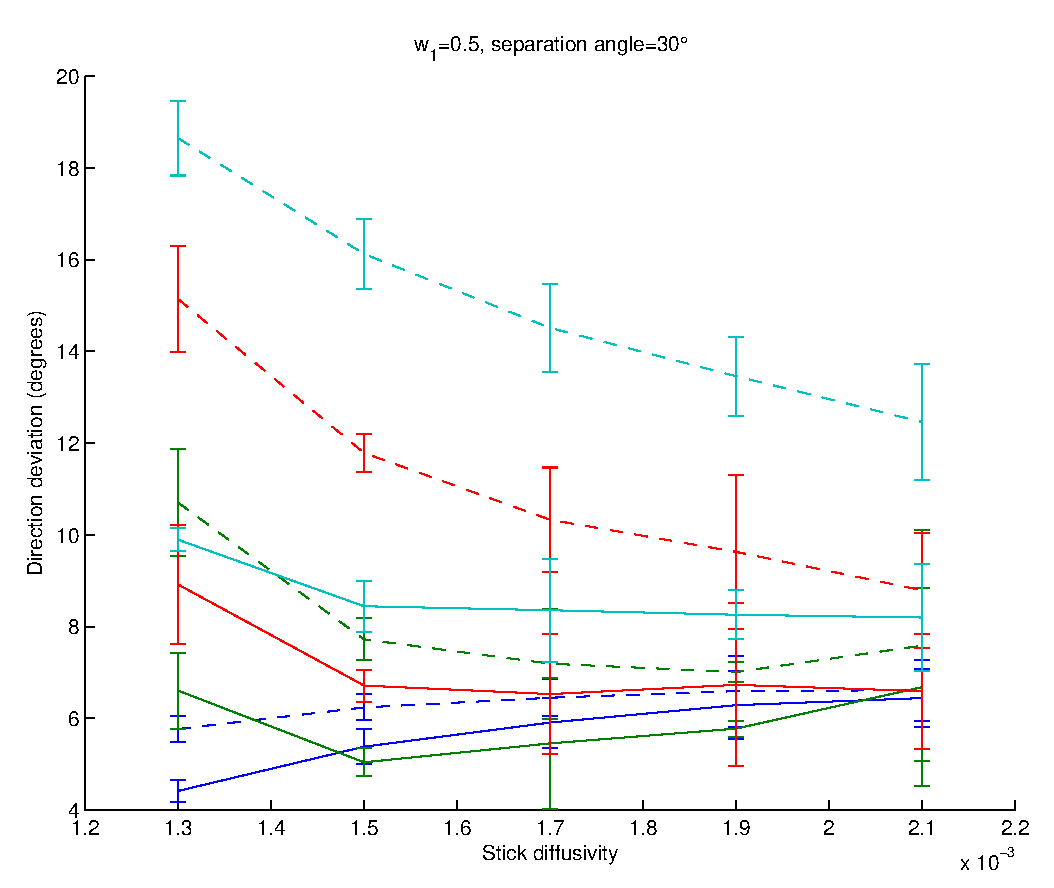
\includegraphics[width=\textwidth]{figures/synth_modbas_weights_diffus__snr=20__w1=5__angle=30.eps}
      \end{subfigure}
      ~
      \begin{subfigure}{0.3\textwidth}
        \centering
        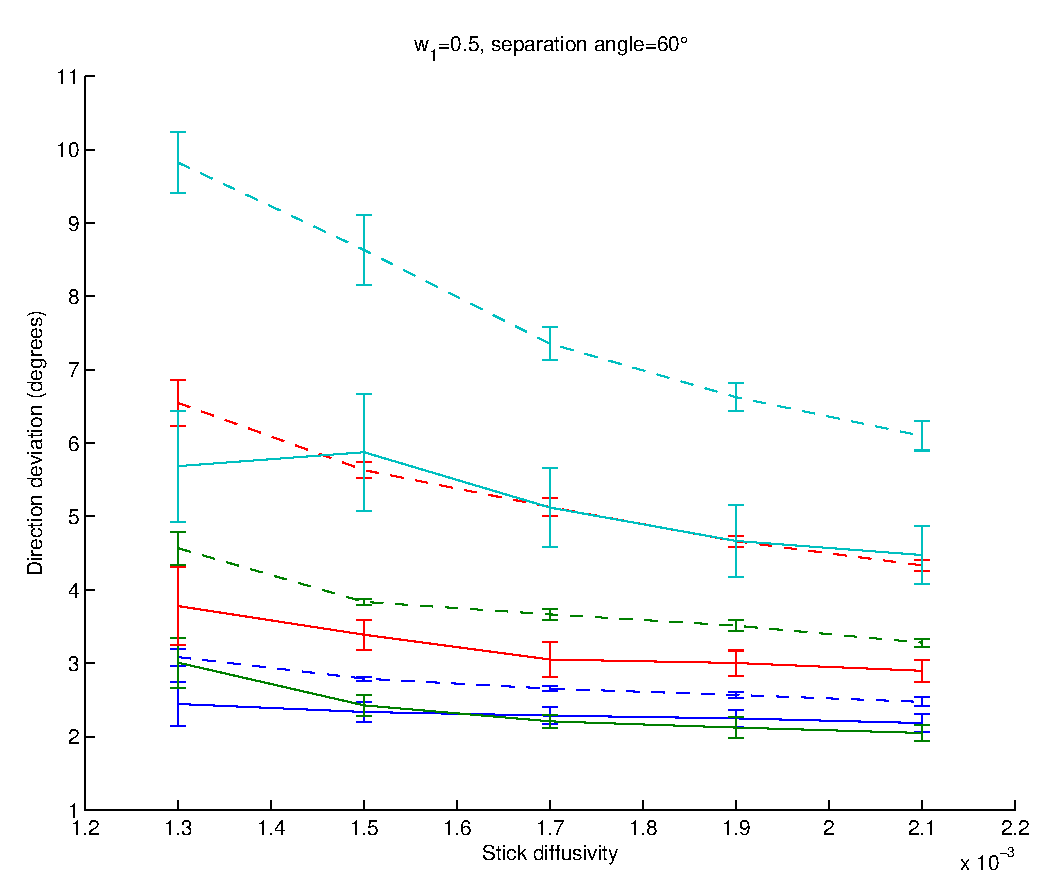
\includegraphics[width=\textwidth]{figures/synth_modbas_weights_diffus__snr=20__w1=5__angle=60.eps}
      \end{subfigure}
      ~
      \begin{subfigure}{0.3\textwidth}
        \centering
        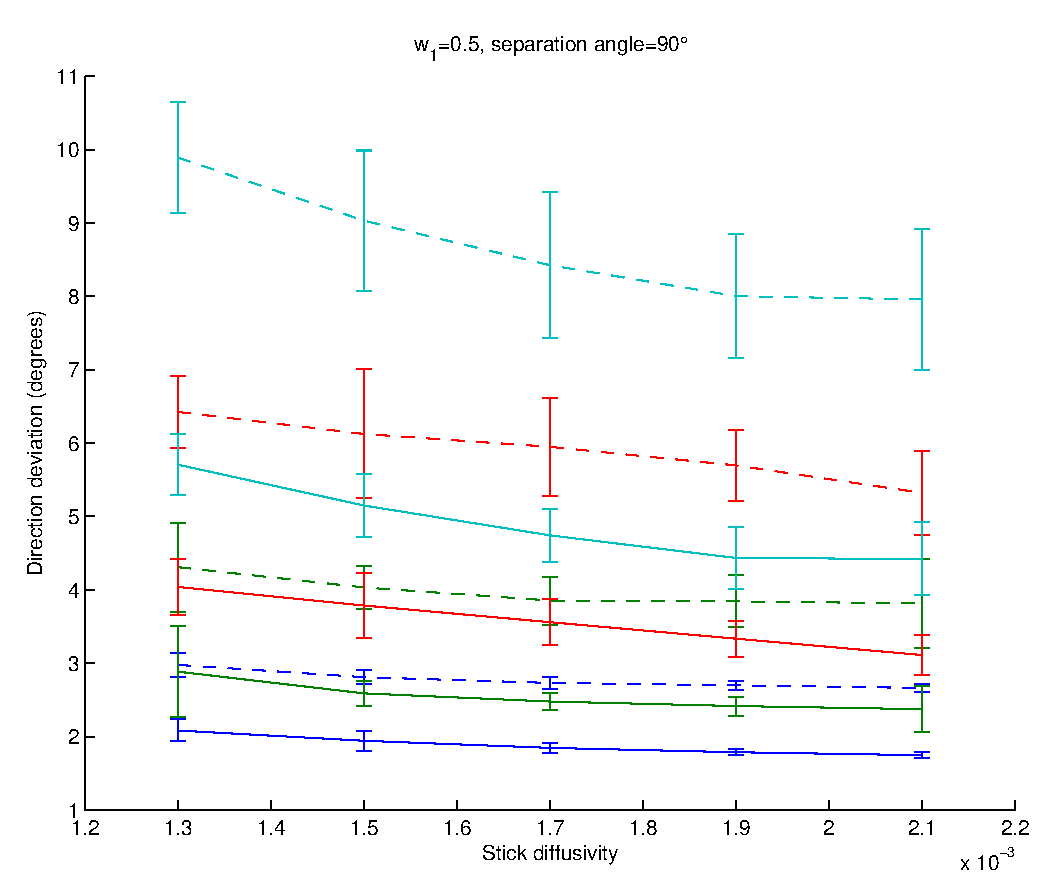
\includegraphics[width=\textwidth]{figures/synth_modbas_weights_diffus__snr=20__w1=5__angle=90.eps}
      \end{subfigure}
  \end{subfigure}
\end{adjustwidth}
  \caption{Estimation results with both weight and diffusivity estimation. From top to bottom: synthesized weights are (0.3, 0.7), (0.4, 0.6), (0.5, 0.5) respectively. From left to right: separation angles are 30, 60 and 90 degrees, respectively. Simulated SNR is 20.}
\end{figure}


\subsubsection{Ball-And-Sticks Model}

\begin{figure}[H]
  \begin{adjustwidth}{-\oddsidemargin}{-\rightmargin}
    \begin{subfigure}{0.8\paperwidth}
      \begin{subfigure}{0.3\textwidth}
        \centering
        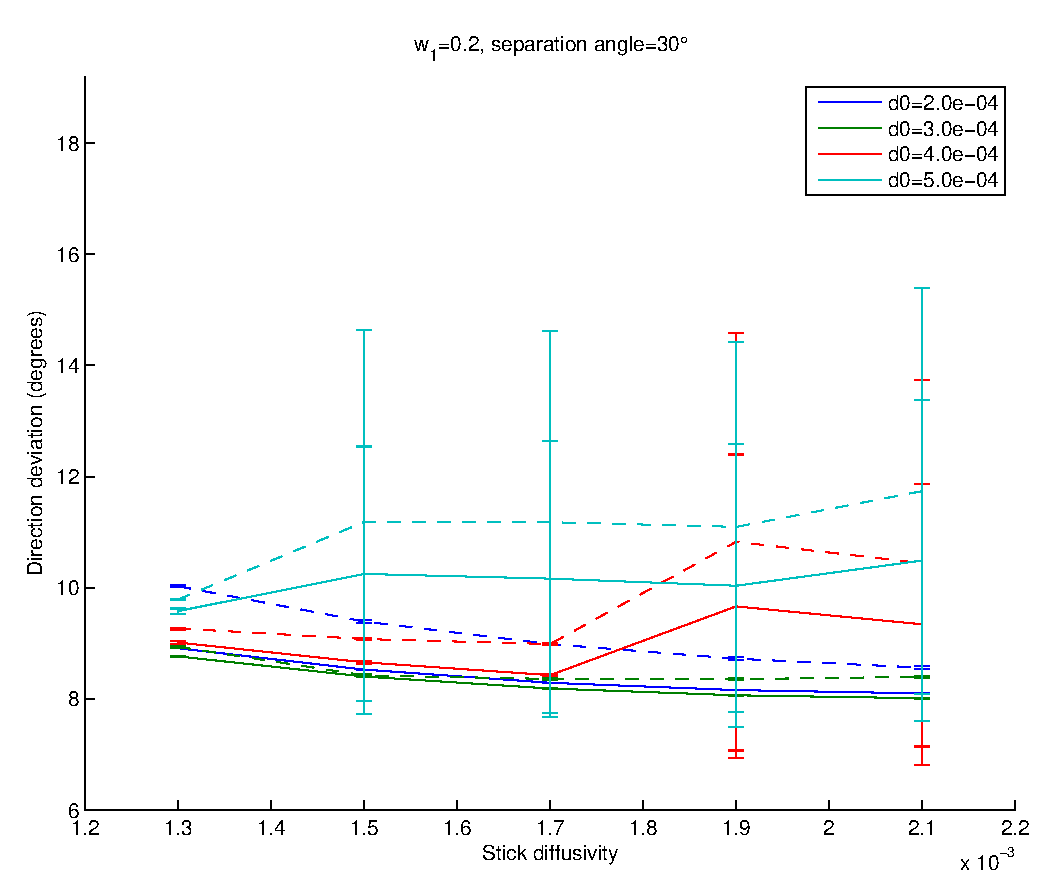
\includegraphics[width=\textwidth]{figures/synth_bas_weights__snr=20__w1=2__angle=30.eps}
      \end{subfigure}
      ~
      \begin{subfigure}{0.3\textwidth}
        \centering
        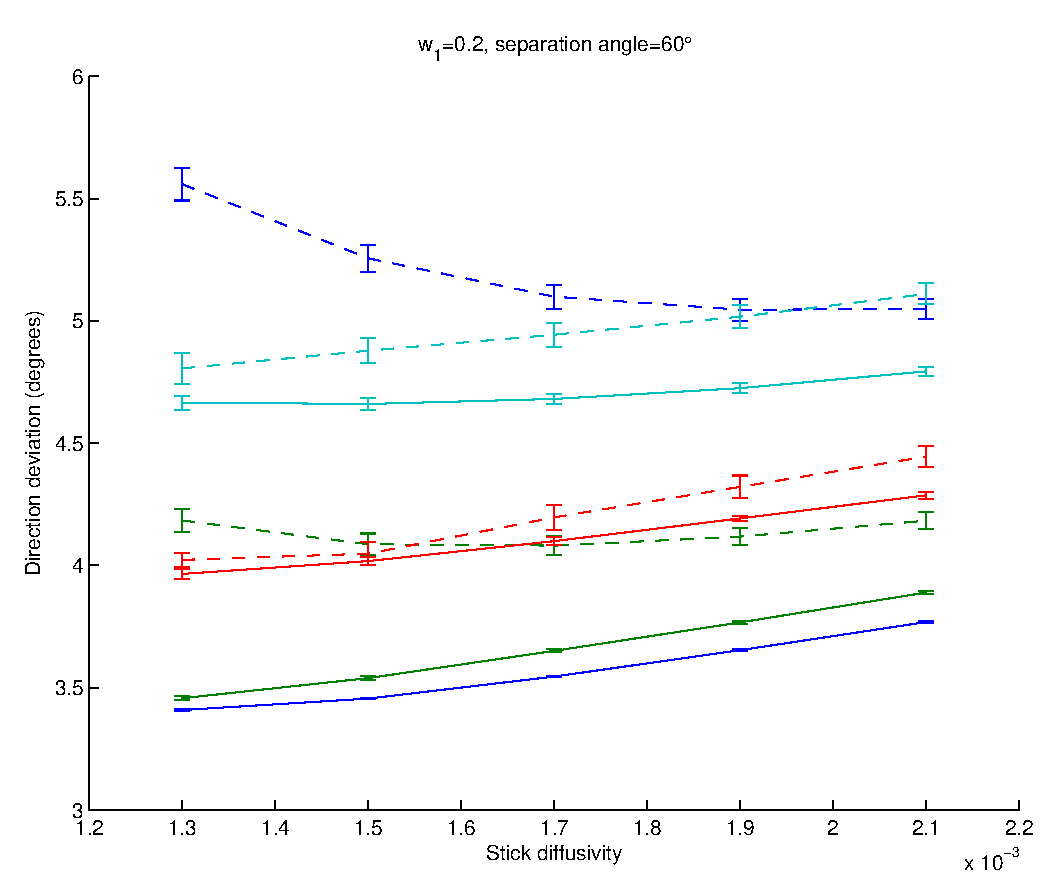
\includegraphics[width=\textwidth]{figures/synth_bas_weights__snr=20__w1=2__angle=60.eps}
      \end{subfigure}
      ~
      \begin{subfigure}{0.3\textwidth}
        \centering
        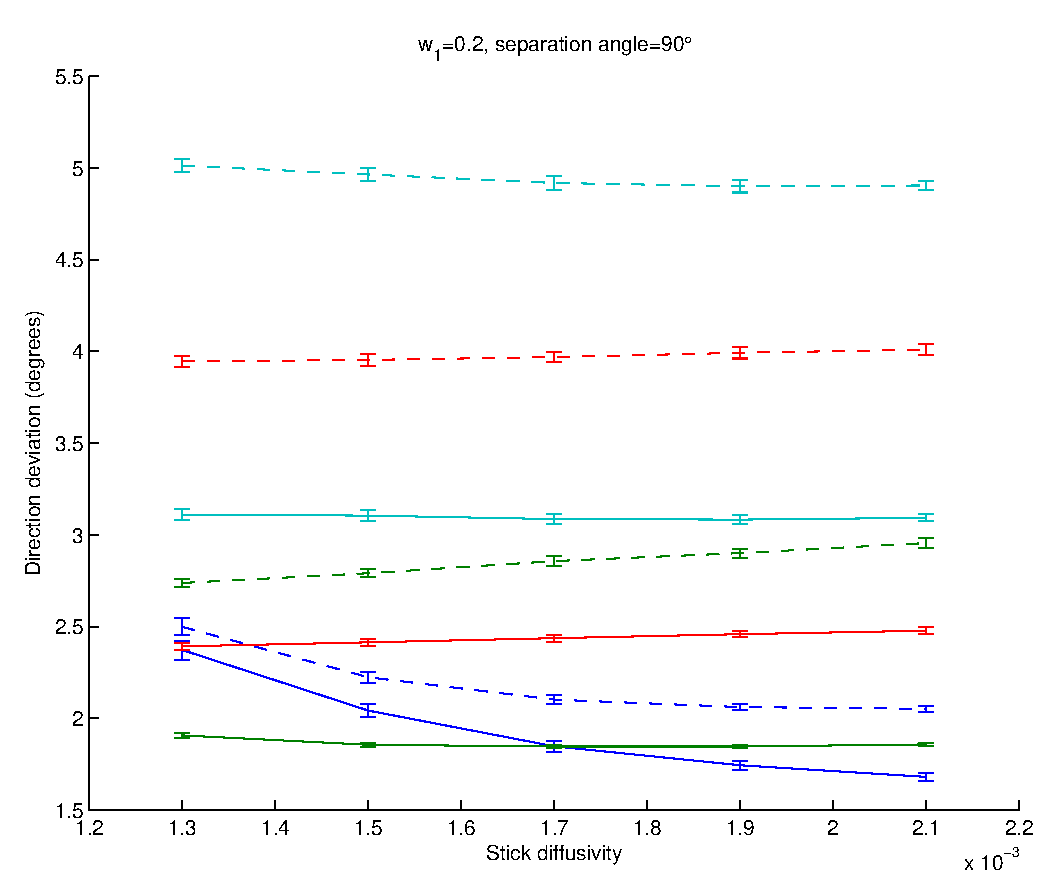
\includegraphics[width=\textwidth]{figures/synth_bas_weights__snr=20__w1=2__angle=90.eps}
      \end{subfigure}
    \end{subfigure}
    
    \begin{subfigure}{0.8\paperwidth}
      \begin{subfigure}{0.3\textwidth}
        \centering
        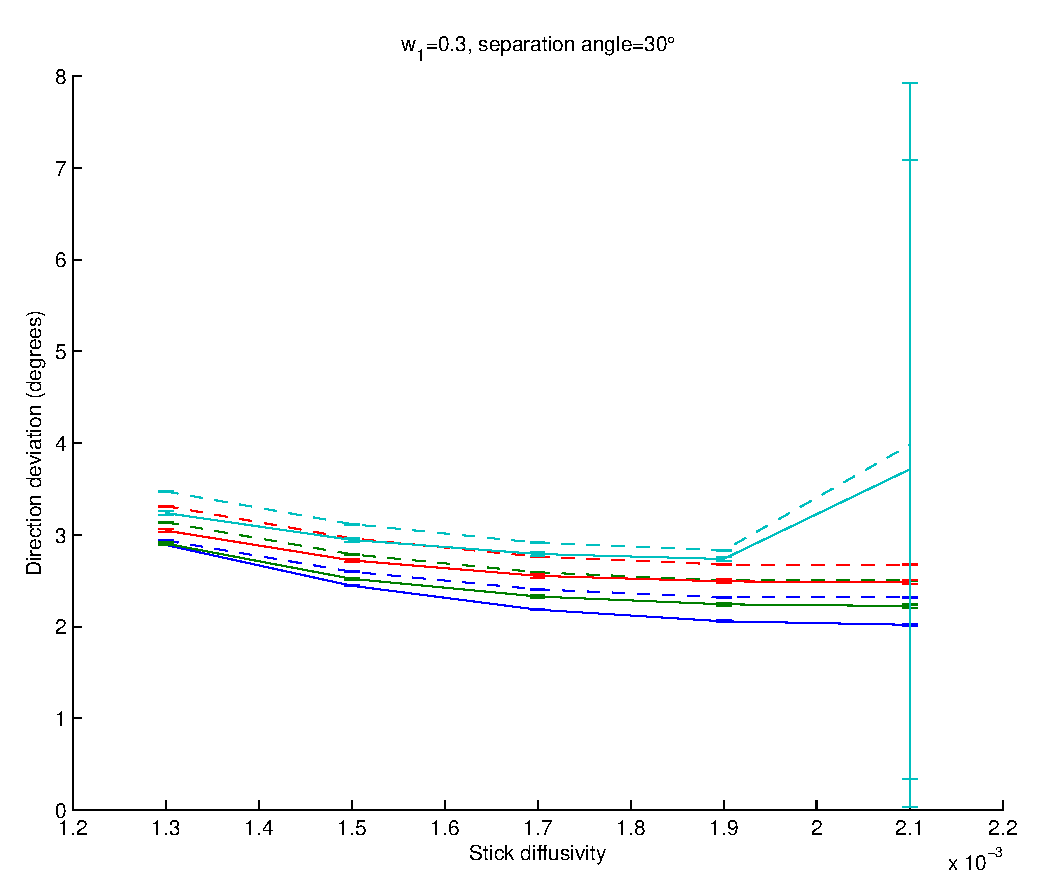
\includegraphics[width=\textwidth]{figures/synth_bas_weights__snr=20__w1=3__angle=30.eps}
      \end{subfigure}
      ~
      \begin{subfigure}{0.3\textwidth}
        \centering
        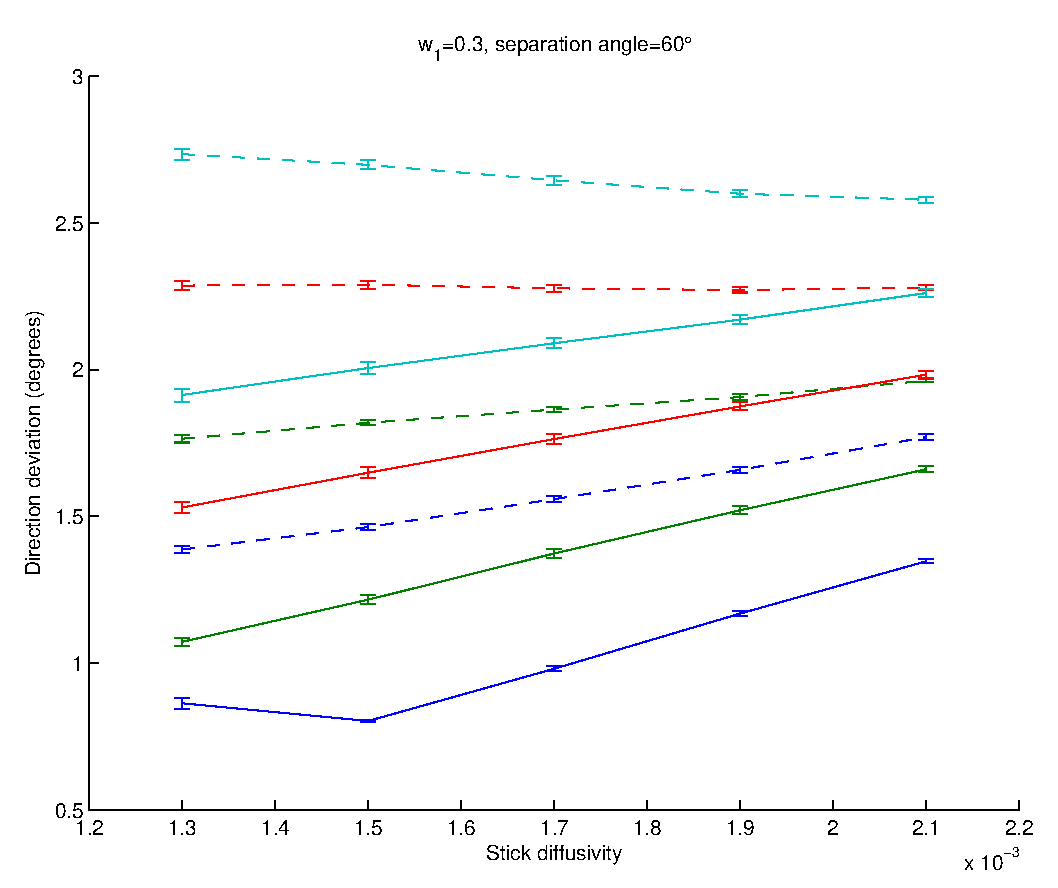
\includegraphics[width=\textwidth]{figures/synth_bas_weights__snr=20__w1=3__angle=60.eps}
      \end{subfigure}
      ~
      \begin{subfigure}{0.3\textwidth}
        \centering
        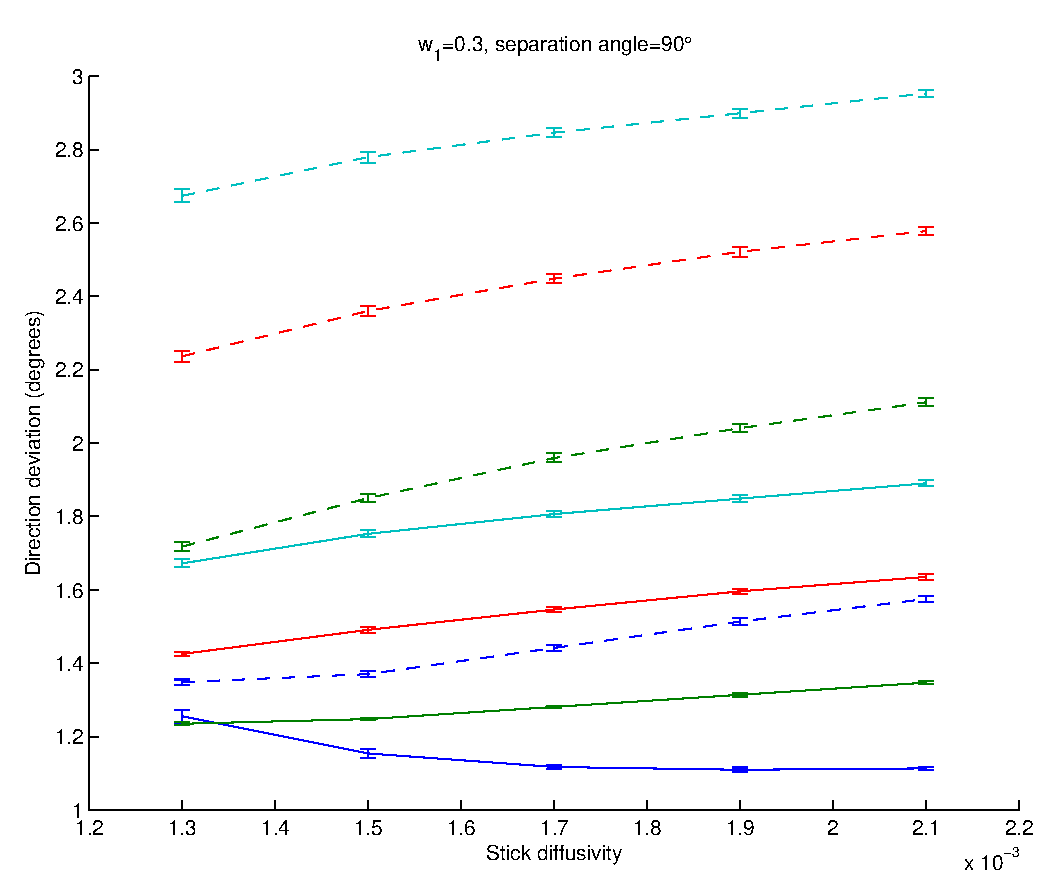
\includegraphics[width=\textwidth]{figures/synth_bas_weights__snr=20__w1=3__angle=90.eps}
      \end{subfigure}
    \end{subfigure}
    \begin{subfigure}{0.8\paperwidth}
      \begin{subfigure}{0.3\textwidth}
        \centering
        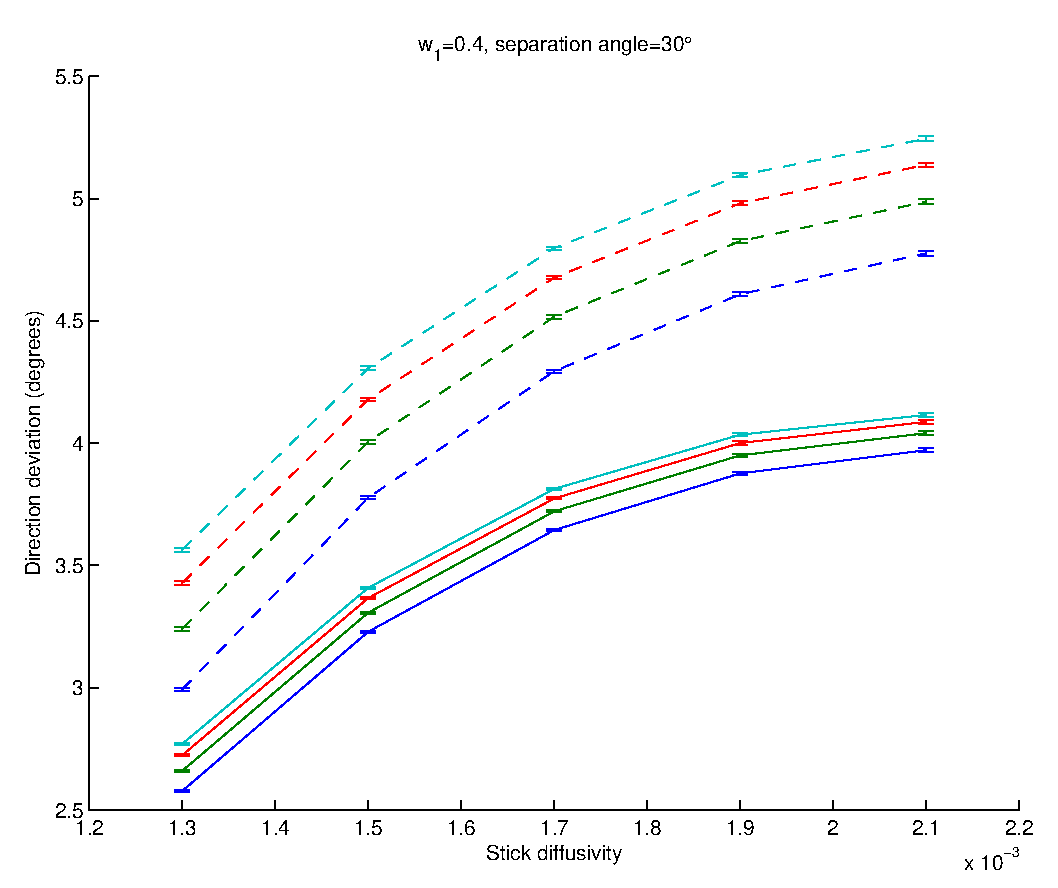
\includegraphics[width=\textwidth]{figures/synth_bas_weights__snr=20__w1=4__angle=30.eps}
      \end{subfigure}
      ~
      \begin{subfigure}{0.3\textwidth}
        \centering
        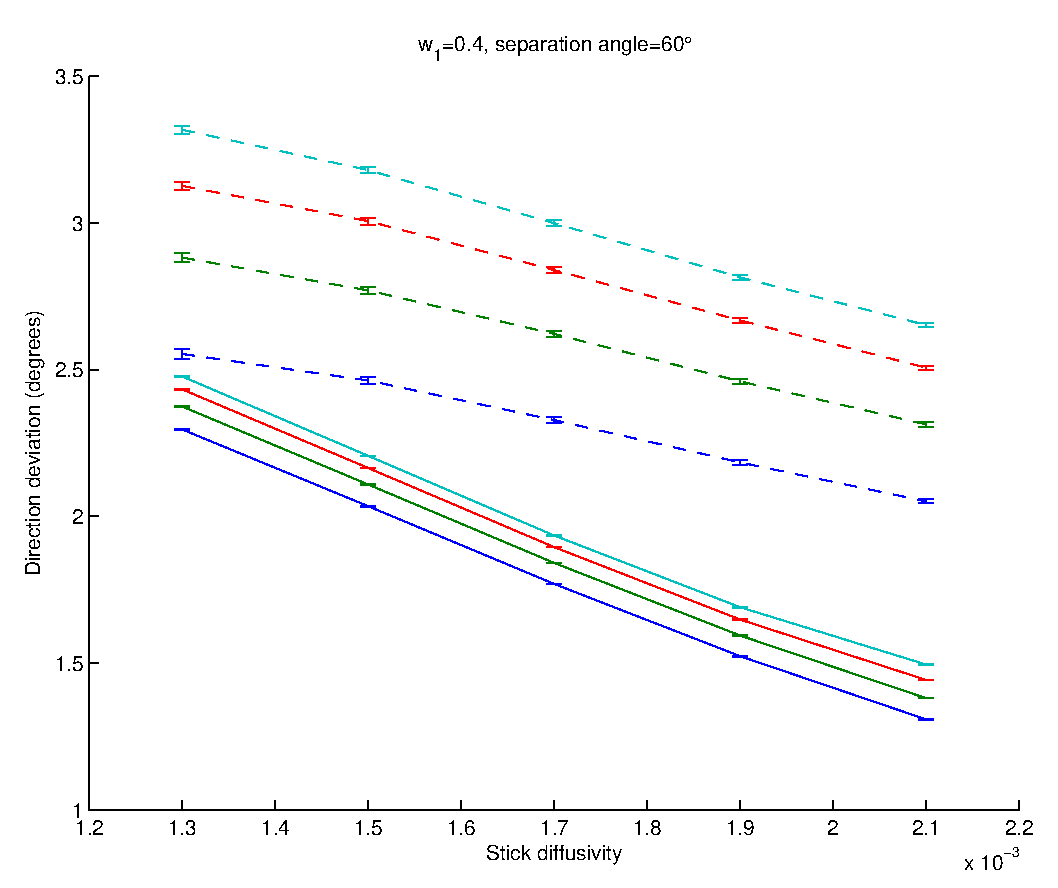
\includegraphics[width=\textwidth]{figures/synth_bas_weights__snr=20__w1=4__angle=60.eps}
      \end{subfigure}
      ~
      \begin{subfigure}{0.3\textwidth}
        \centering
        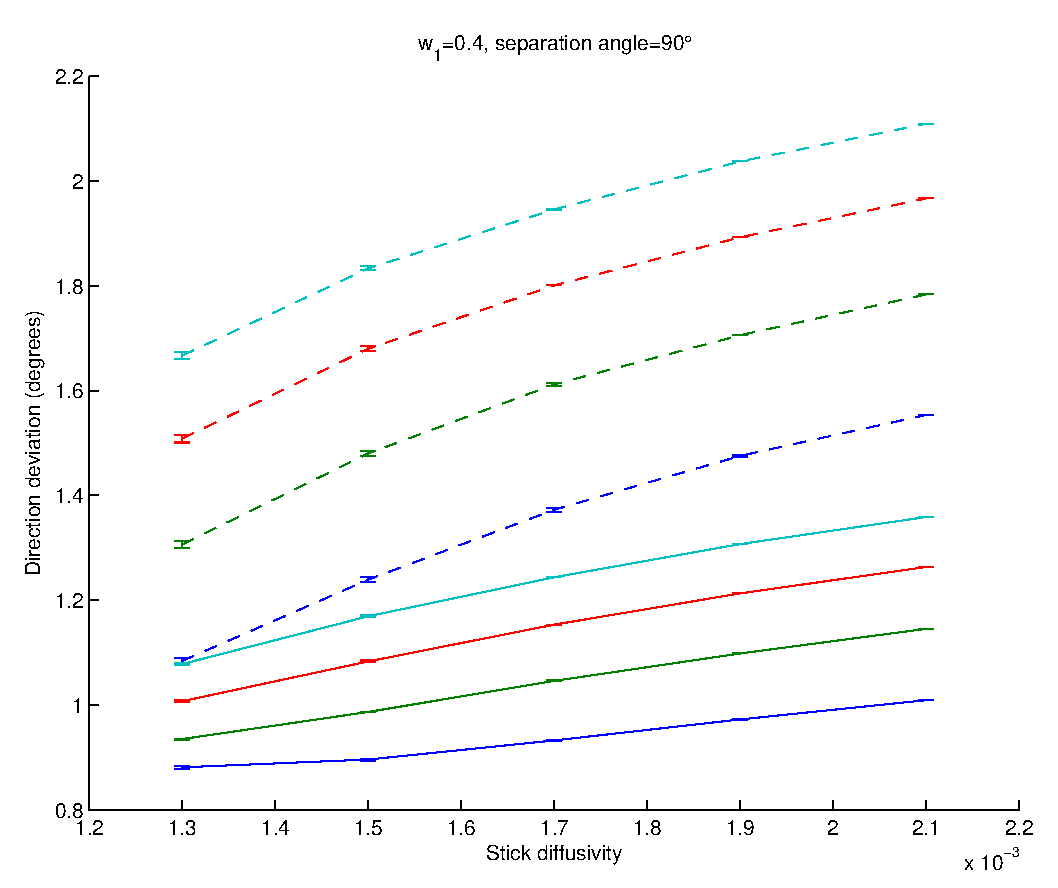
\includegraphics[width=\textwidth]{figures/synth_bas_weights__snr=20__w1=4__angle=90.eps}
      \end{subfigure}
    \end{subfigure}
  \end{adjustwidth}
  
  \caption{Estimation results with weight estimation. Stick diffusivities are fixed at $1.7\times 10^{-3}$, ball diffusivity at $3.0\times 10^{-4}$. From top to bottom: synthesized weights are (0.2, 0.2, 0.6), (0.3, 0.3, 0.4), (0.4, 0.4, 0.2) respectively. From left to right: separation angles are 30, 60 and 90 degrees, respectively. Simulated SNR is 20.}
\end{figure}

\begin{figure}[H]
  \begin{adjustwidth}{-\oddsidemargin}{-\rightmargin}
    \begin{subfigure}{0.8\paperwidth}
      \begin{subfigure}{0.3\textwidth}
        \centering
        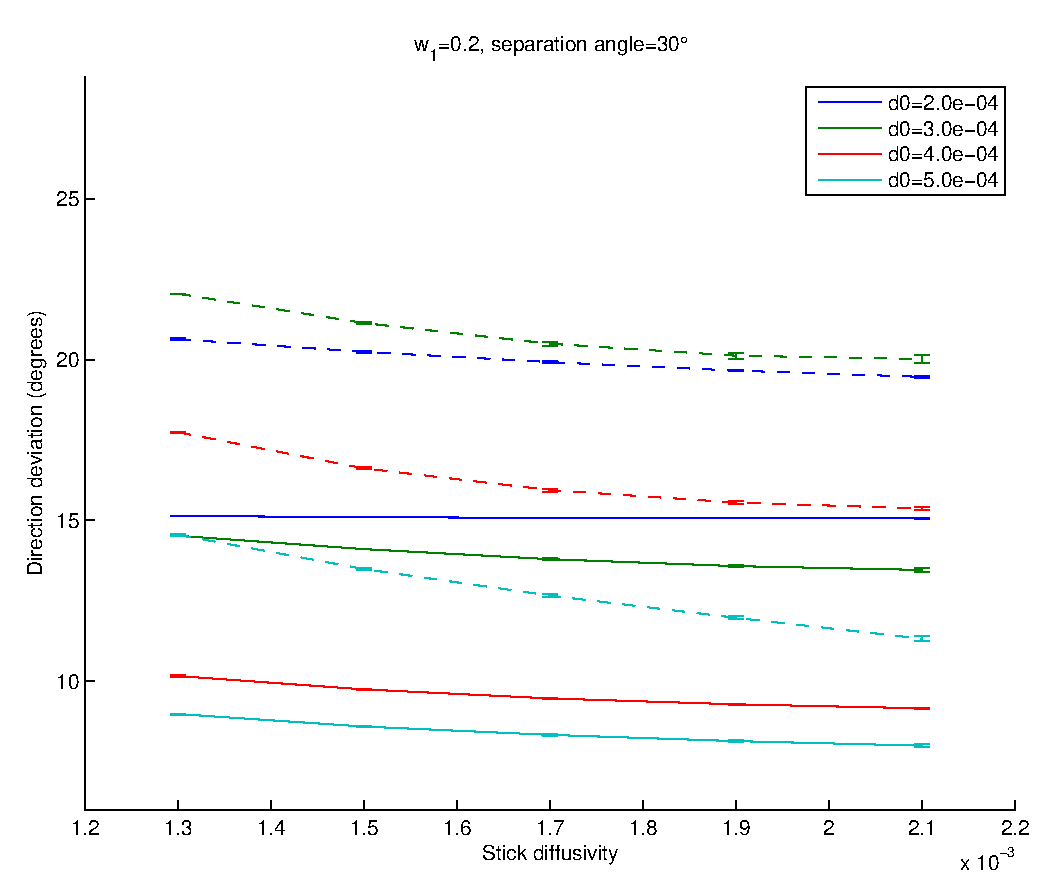
\includegraphics[width=\textwidth]{figures/synth_bas_diffus__snr=20__w1=2__angle=30.eps}
      \end{subfigure}
      ~
      \begin{subfigure}{0.3\textwidth}
        \centering
        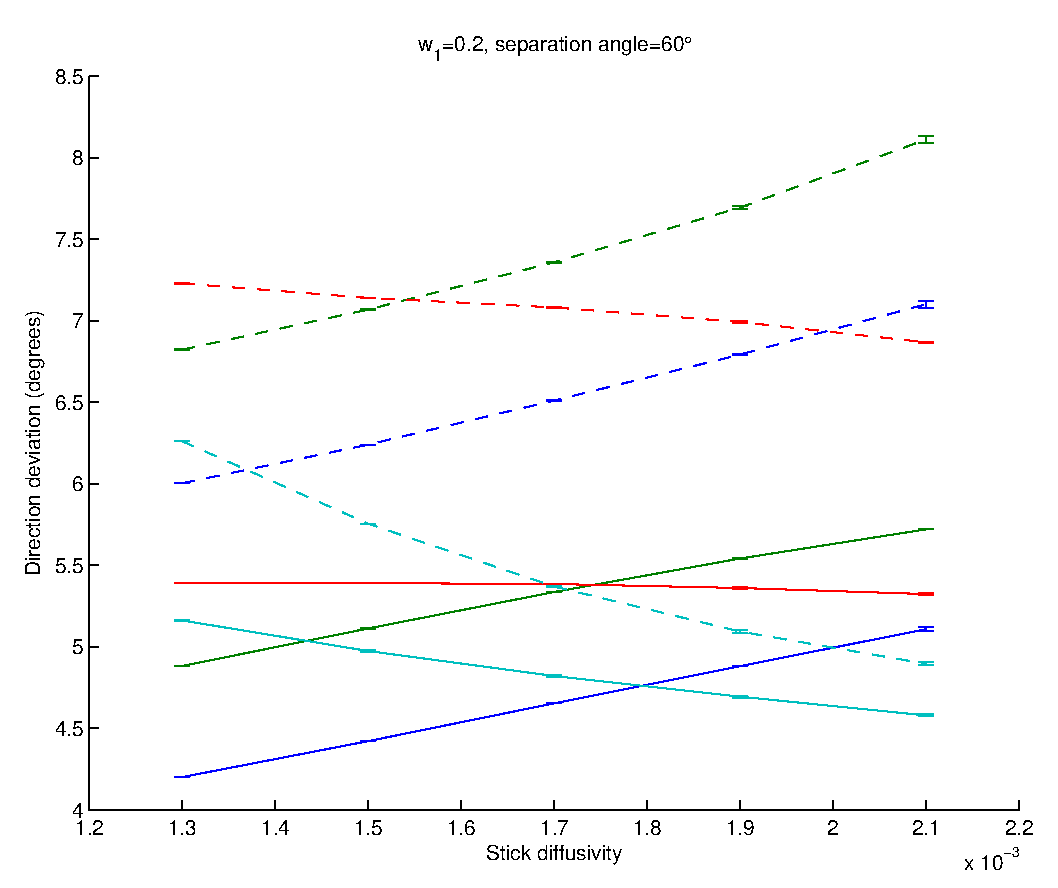
\includegraphics[width=\textwidth]{figures/synth_bas_diffus__snr=20__w1=2__angle=60.eps}
      \end{subfigure}
      ~
      \begin{subfigure}{0.3\textwidth}
        \centering
        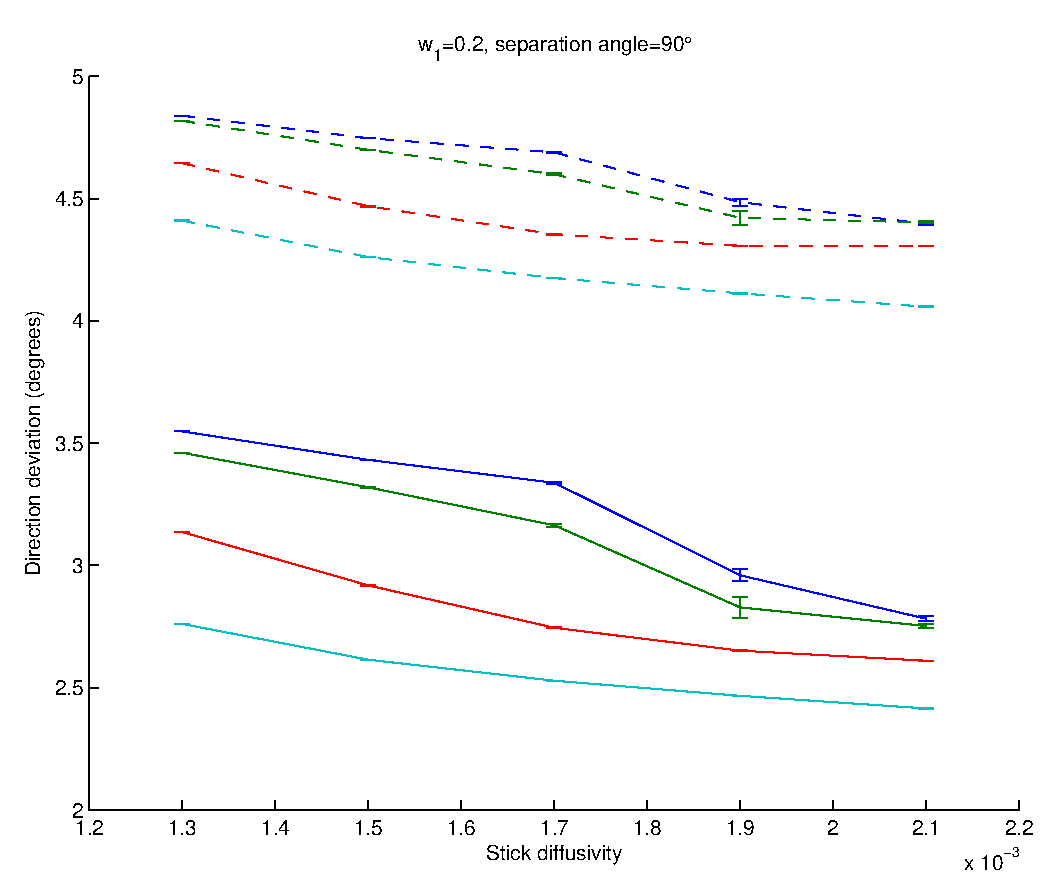
\includegraphics[width=\textwidth]{figures/synth_bas_diffus__snr=20__w1=2__angle=90.eps}
      \end{subfigure}
    \end{subfigure}
    
    \begin{subfigure}{0.8\paperwidth}
      \begin{subfigure}{0.3\textwidth}
        \centering
        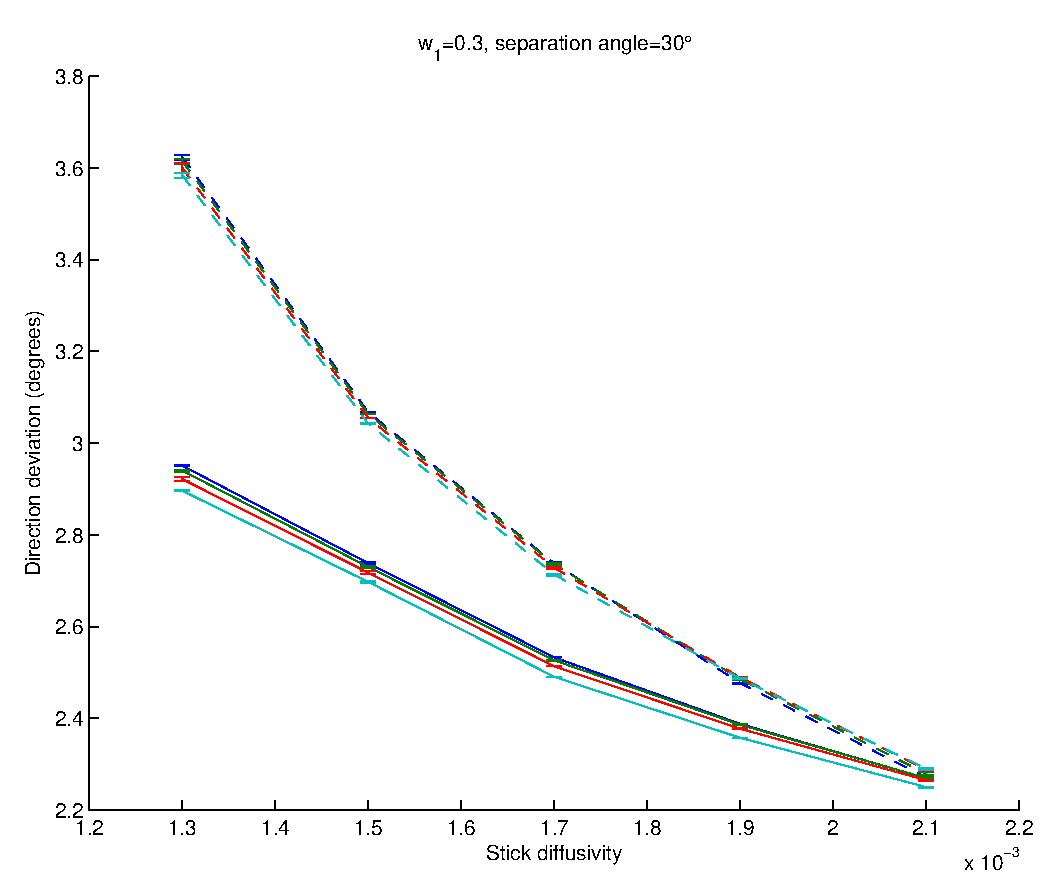
\includegraphics[width=\textwidth]{figures/synth_bas_diffus__snr=20__w1=3__angle=30.eps}
      \end{subfigure}
      ~
      \begin{subfigure}{0.3\textwidth}
        \centering
        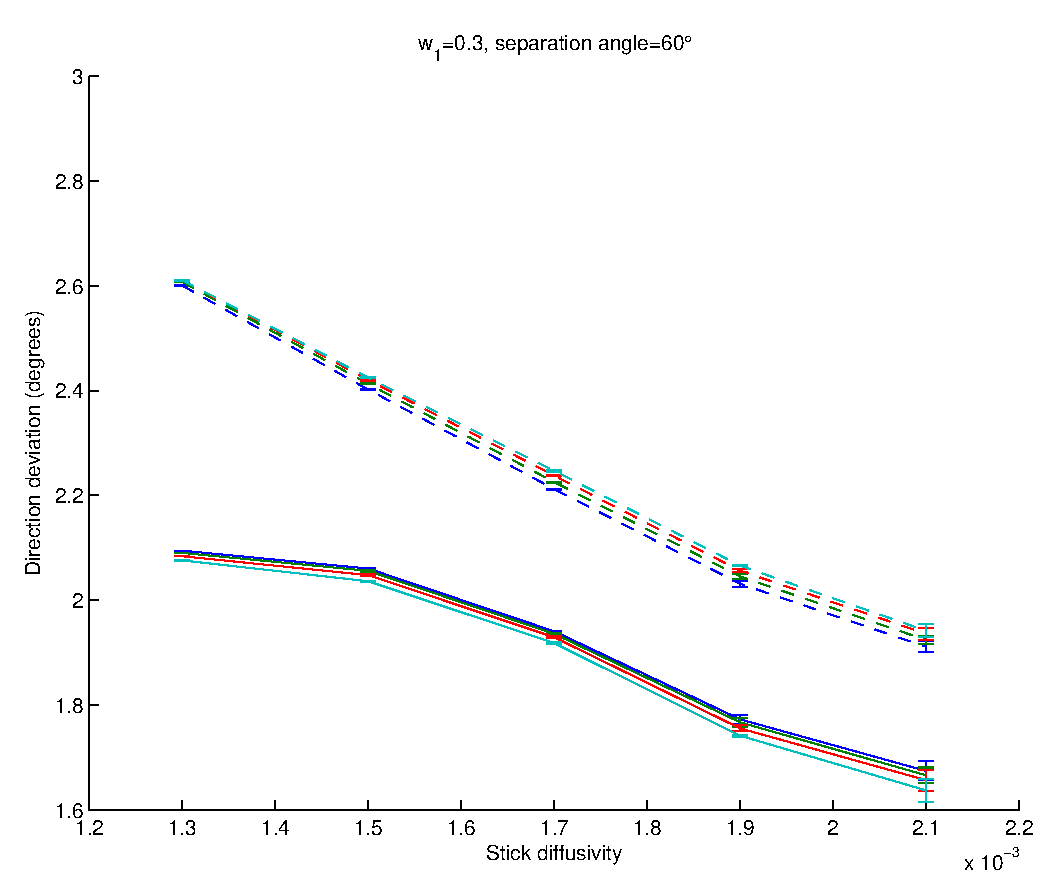
\includegraphics[width=\textwidth]{figures/synth_bas_diffus__snr=20__w1=3__angle=60.eps}
      \end{subfigure}
      ~
      \begin{subfigure}{0.3\textwidth}
        \centering
        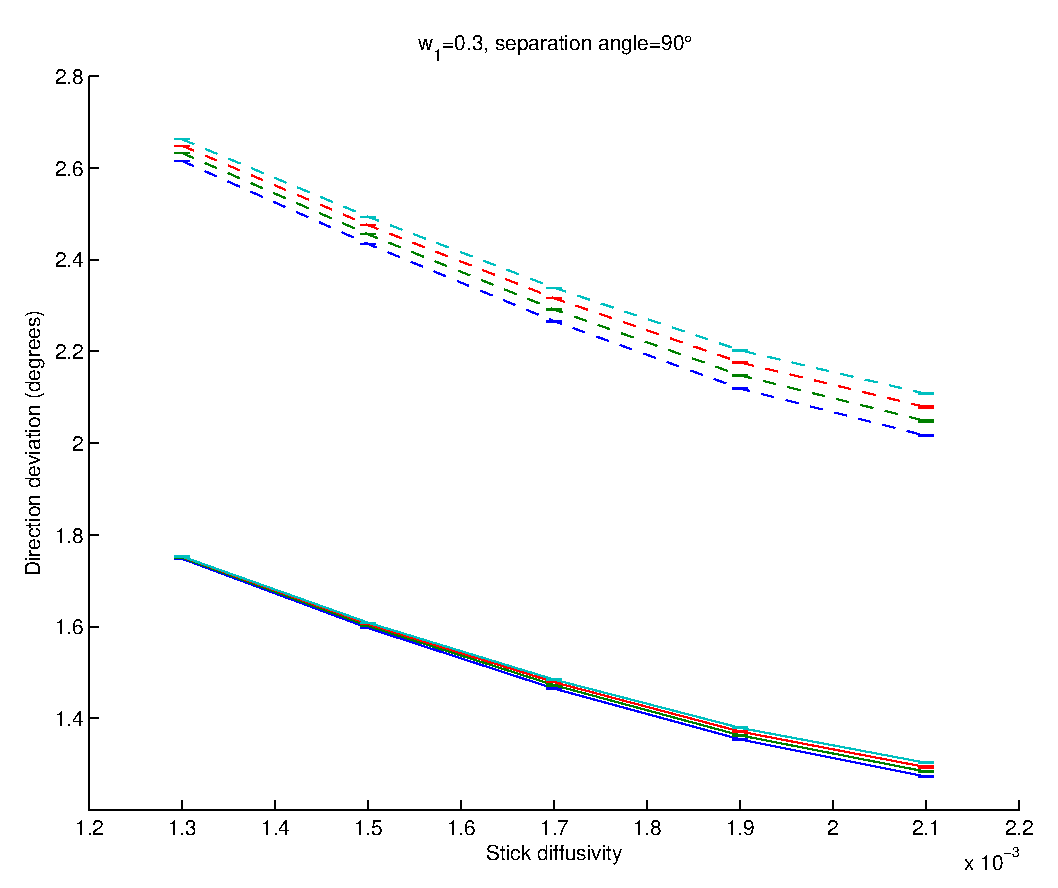
\includegraphics[width=\textwidth]{figures/synth_bas_diffus__snr=20__w1=3__angle=90.eps}
      \end{subfigure}
    \end{subfigure}
    \begin{subfigure}{0.8\paperwidth}
      \begin{subfigure}{0.3\textwidth}
        \centering
        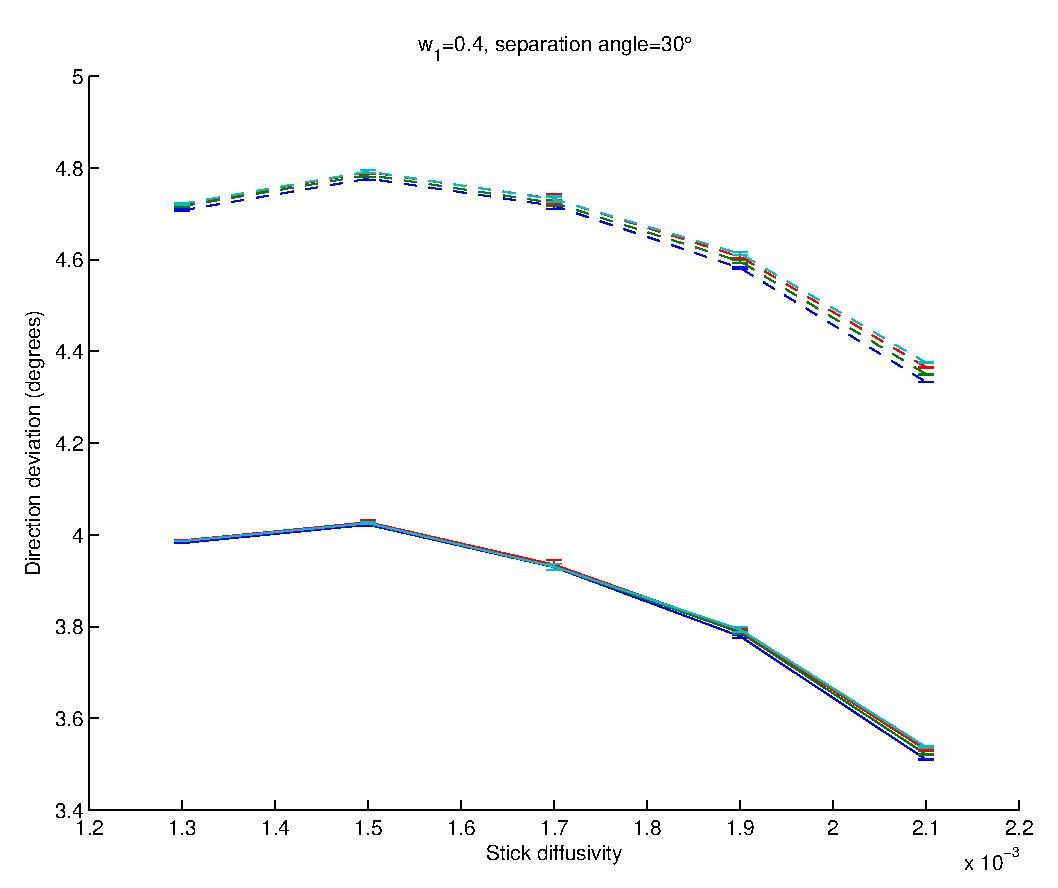
\includegraphics[width=\textwidth]{figures/synth_bas_diffus__snr=20__w1=4__angle=30.eps}
      \end{subfigure}
      ~
      \begin{subfigure}{0.3\textwidth}
        \centering
        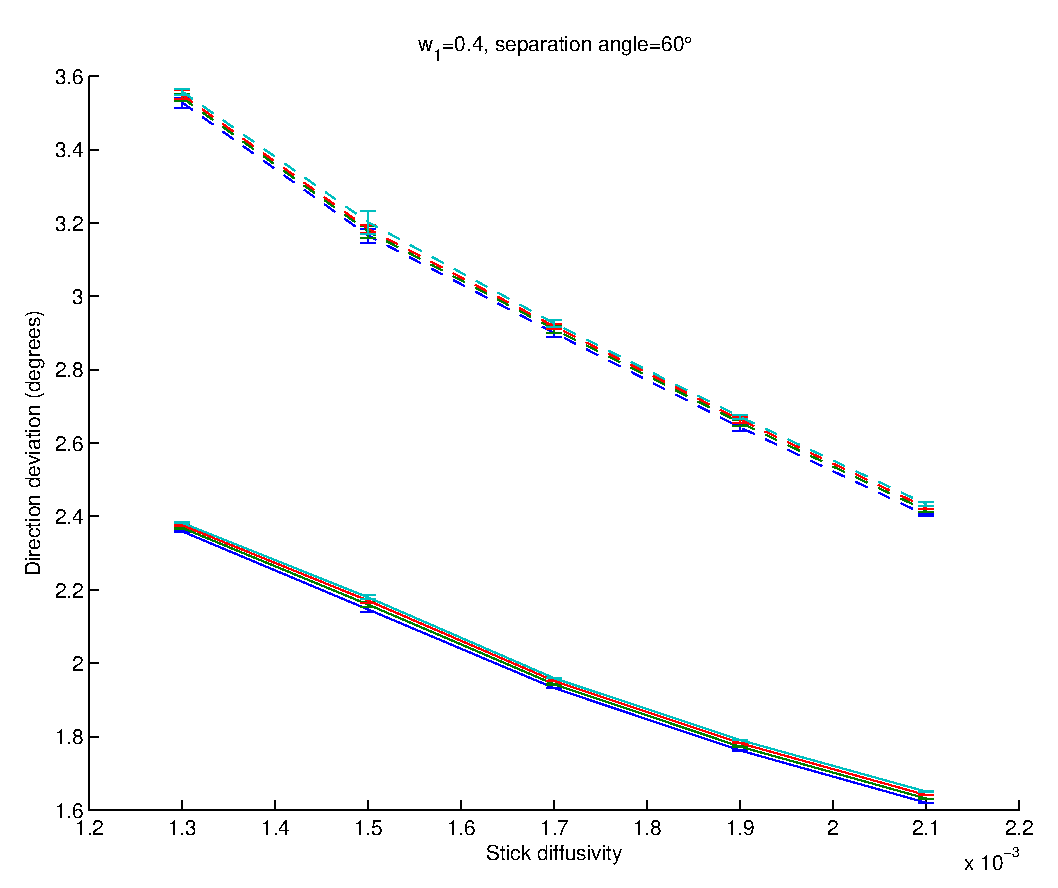
\includegraphics[width=\textwidth]{figures/synth_bas_diffus__snr=20__w1=4__angle=60.eps}
      \end{subfigure}
      ~
      \begin{subfigure}{0.3\textwidth}
        \centering
        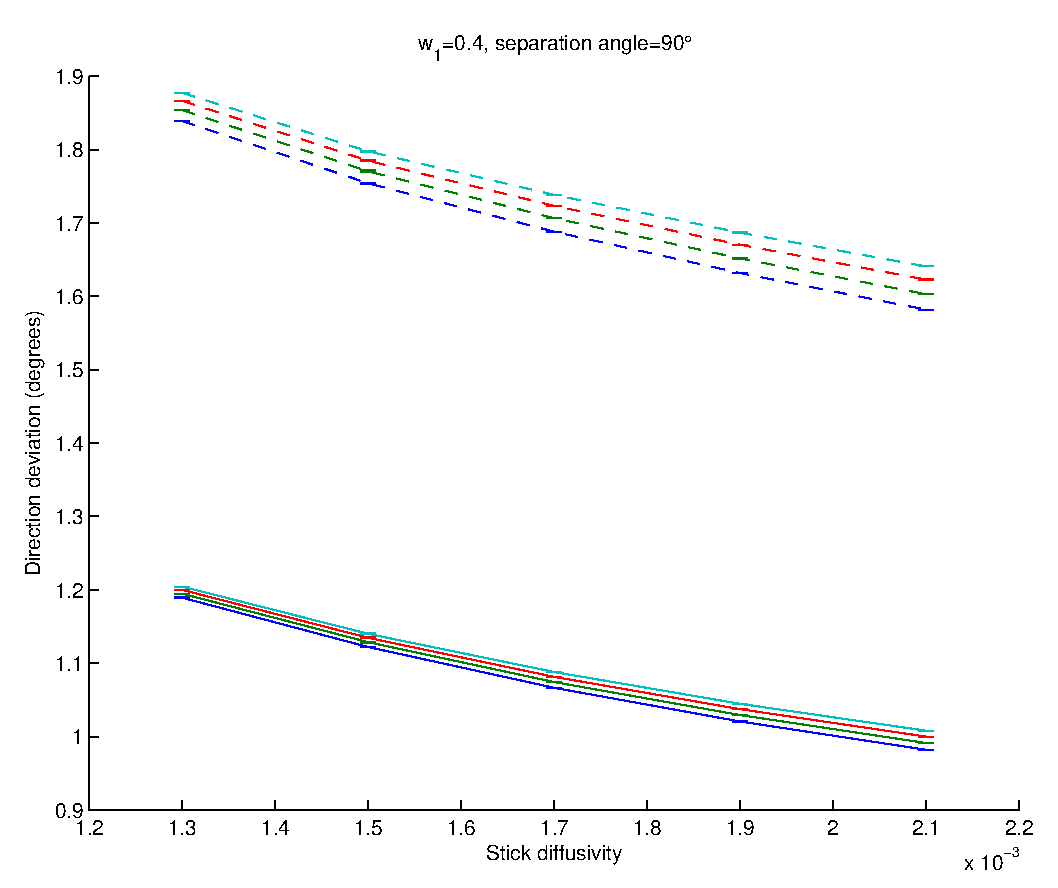
\includegraphics[width=\textwidth]{figures/synth_bas_diffus__snr=20__w1=4__angle=90.eps}
      \end{subfigure}
    \end{subfigure}
  \end{adjustwidth}
  
  \caption{Estimation results with diffusivity estimation. Weights are fixed at (0.3, 0.3, 0.3). From top to bottom: synthesized weights are (0.2, 0.2, 0.6), (0.3, 0.3, 0.4), (0.4, 0.4, 0.2) respectively. From left to right: separation angles are 30, 60 and 90 degrees, respectively. Simulated SNR is 20.}
\end{figure}

\begin{figure}[H]
  \begin{adjustwidth}{-\oddsidemargin}{-\rightmargin}
    \begin{subfigure}{0.8\paperwidth}
      \begin{subfigure}{0.3\textwidth}
        \centering
        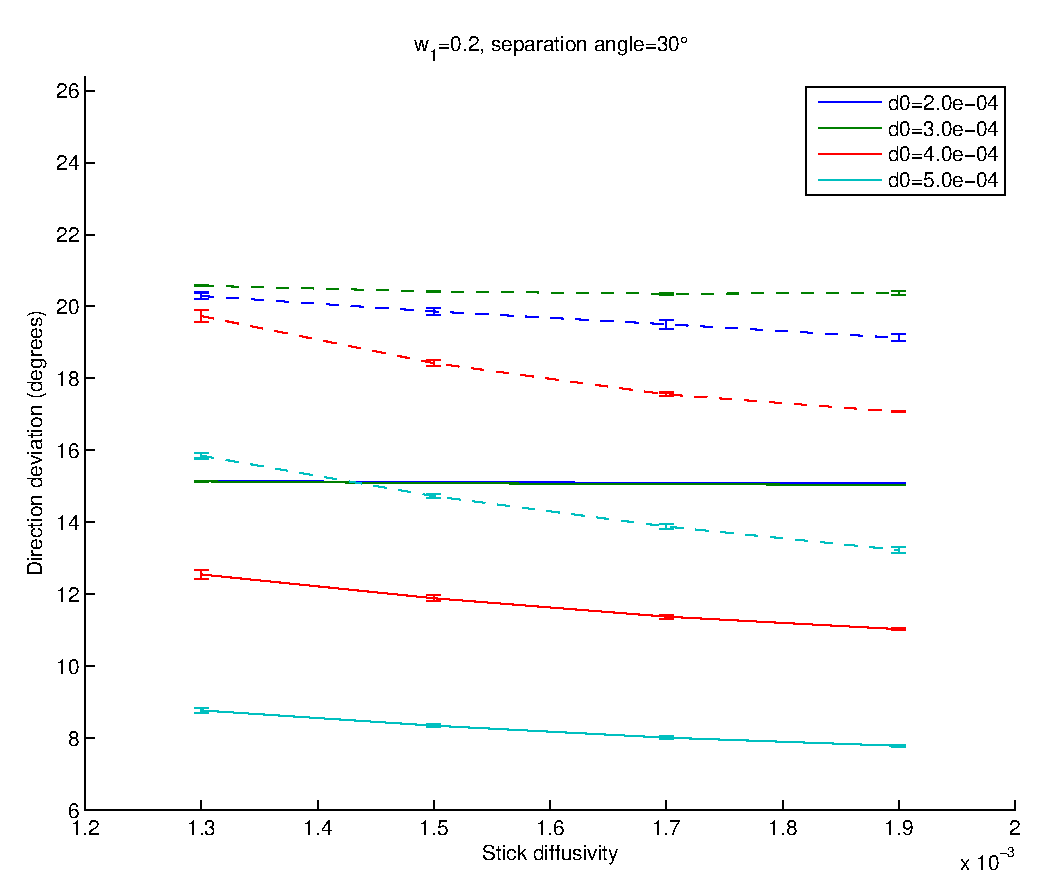
\includegraphics[width=\textwidth]{figures/synth_bas_weights_diffus__snr=20__w1=2__angle=30.eps}
      \end{subfigure}
      ~
      \begin{subfigure}{0.3\textwidth}
        \centering
        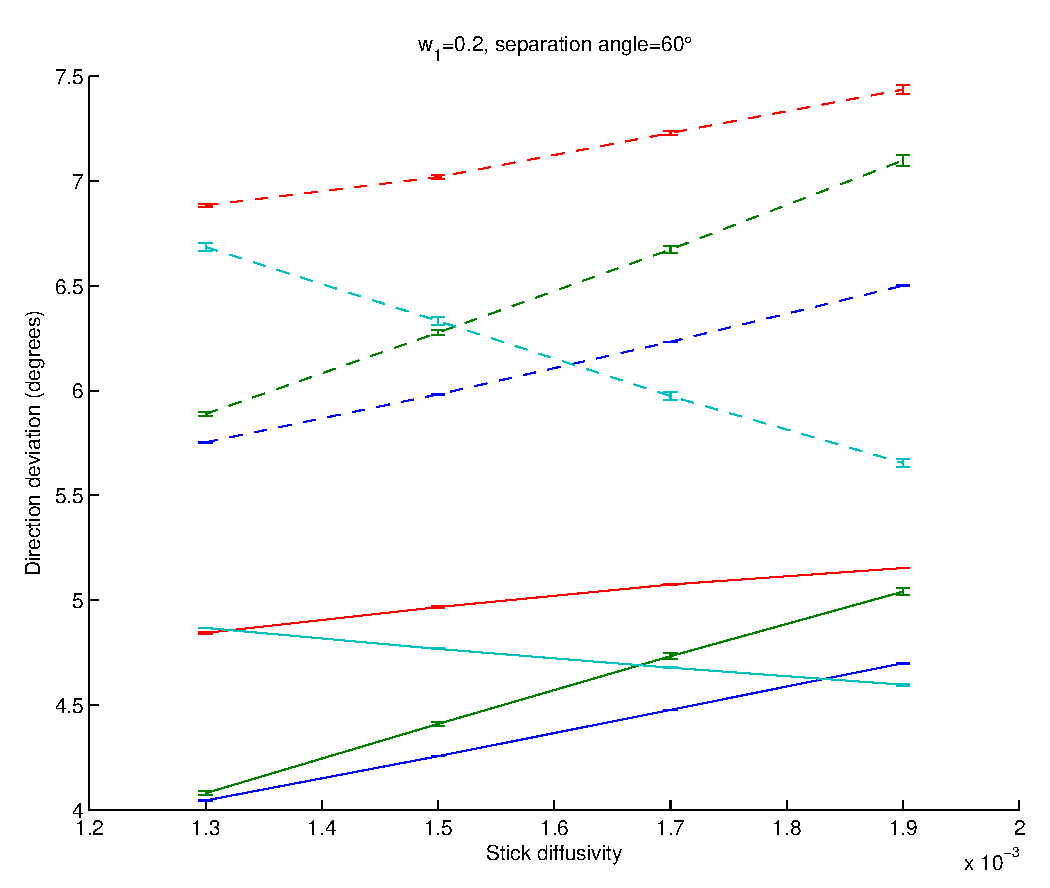
\includegraphics[width=\textwidth]{figures/synth_bas_weights_diffus__snr=20__w1=2__angle=60.eps}
      \end{subfigure}
      ~
      \begin{subfigure}{0.3\textwidth}
        \centering
        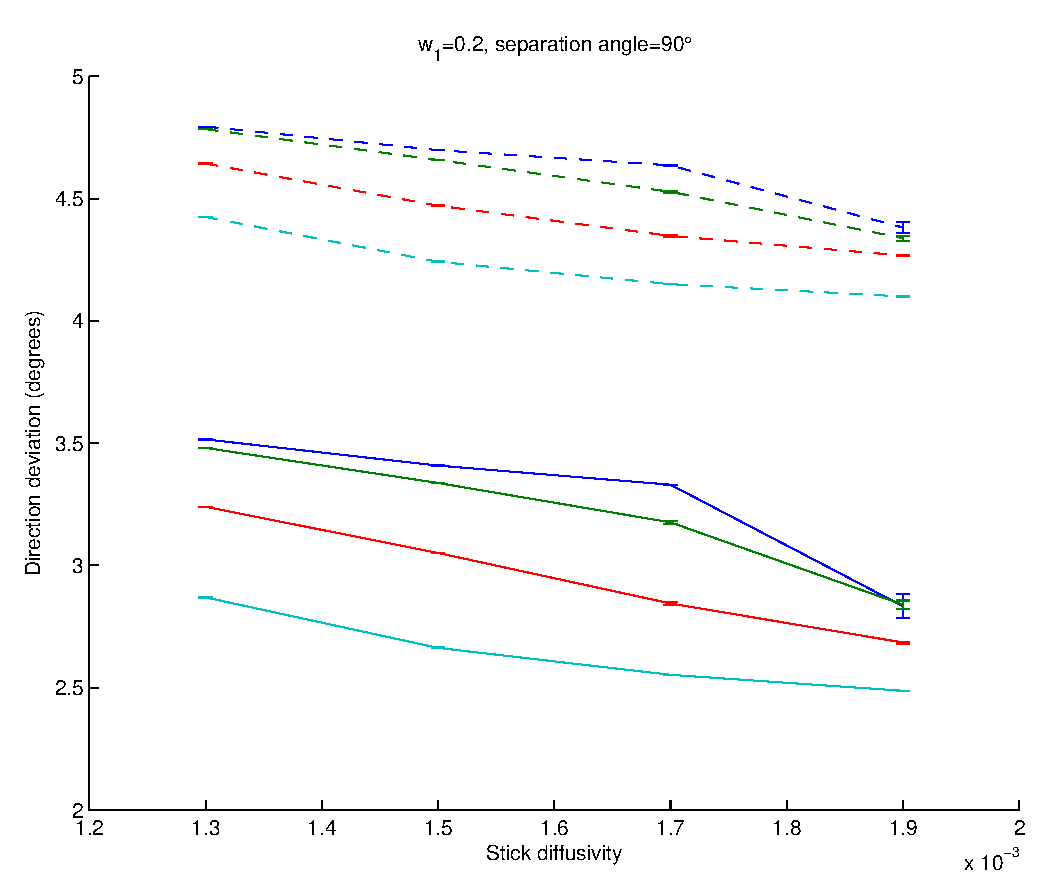
\includegraphics[width=\textwidth]{figures/synth_bas_weights_diffus__snr=20__w1=2__angle=90.eps}
      \end{subfigure}
  \end{subfigure}

  \begin{subfigure}{0.8\paperwidth}
    \begin{subfigure}{0.3\textwidth}
      \centering
      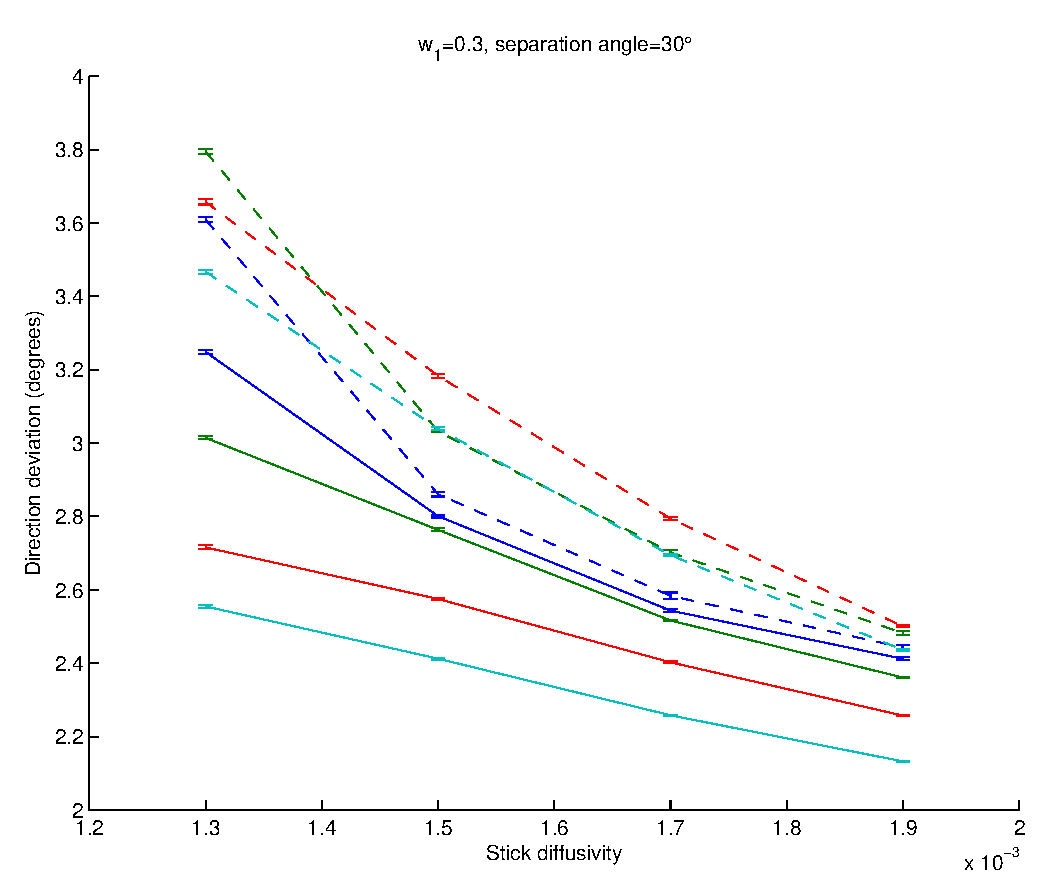
\includegraphics[width=\textwidth]{figures/synth_bas_weights_diffus__snr=20__w1=3__angle=30.eps}
    \end{subfigure}
      ~
      \begin{subfigure}{0.3\textwidth}
        \centering
        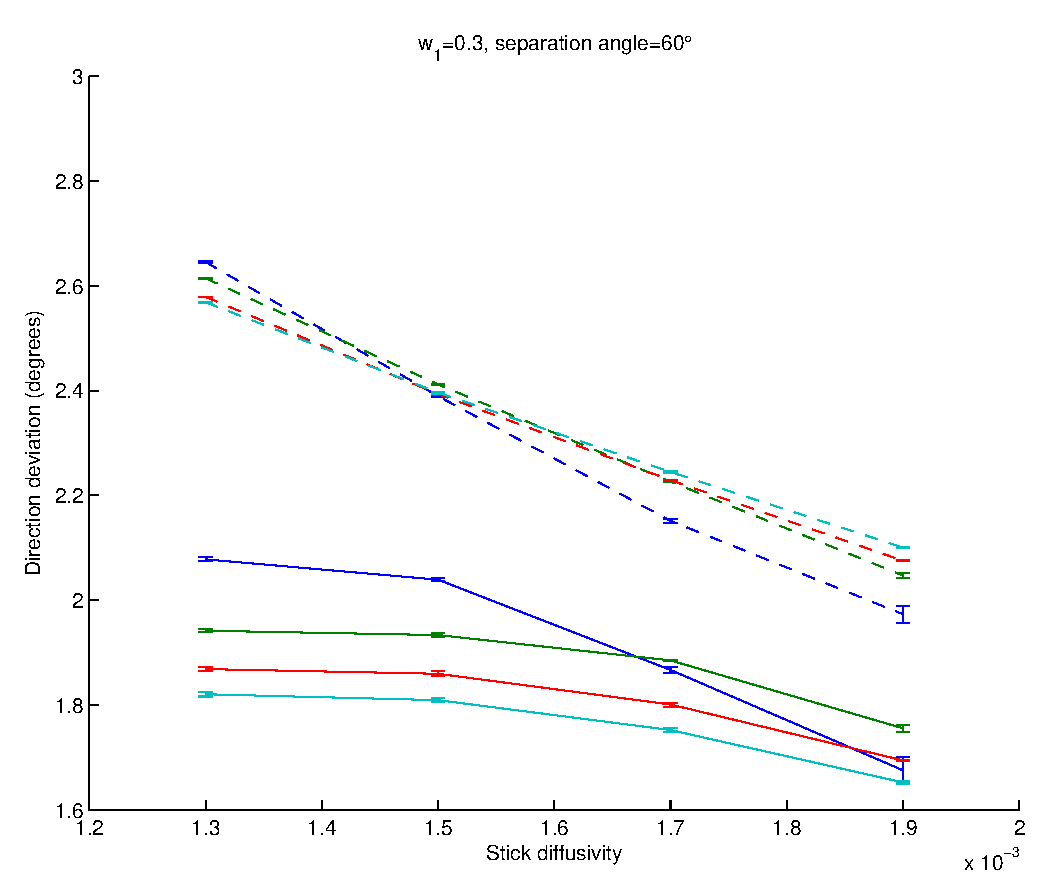
\includegraphics[width=\textwidth]{figures/synth_bas_weights_diffus__snr=20__w1=3__angle=60.eps}
      \end{subfigure}
      ~
      \begin{subfigure}{0.3\textwidth}
        \centering
        \includegraphics[width=\textwidth]{figures/synth_bas_weights_diffus__snr=20__w1=3__angle=90.eps}
      \end{subfigure}
  \end{subfigure}
  \begin{subfigure}{0.8\paperwidth}
      \begin{subfigure}{0.3\textwidth}
        \centering
        \includegraphics[width=\textwidth]{figures/synth_bas_weights_diffus__snr=20__w1=4__angle=30.eps}
      \end{subfigure}
      ~
      \begin{subfigure}{0.3\textwidth}
        \centering
        \includegraphics[width=\textwidth]{figures/synth_bas_weights_diffus__snr=20__w1=4__angle=60.eps}
      \end{subfigure}
      ~
      \begin{subfigure}{0.3\textwidth}
        \centering
        \includegraphics[width=\textwidth]{figures/synth_bas_weights_diffus__snr=20__w1=4__angle=90.eps}
      \end{subfigure}
  \end{subfigure}
\end{adjustwidth}
  \caption{Estimation results with both weight and diffusivity estimation. From top to bottom: synthesized weights are (0.2, 0.2, 0.6), (0.3, 0.3, 0.4), (0.4, 0.4, 0.2) respectively. From left to right: separation angles are 30, 60 and 90 degrees, respectively. Simulated SNR is 20.}
\end{figure}

\subsection{Phantom data}

This section presents estimation results of the MICCAI Fiber Cup phantom data. For each voxel estimation is performed 20 times with random fiber direction initialization. In figures below the plotted fiber directions at each voxel are chosen randomly from the 20 estimation results. Statistics of the likelihood value at termination are shown below the fiber directions.

\subsubsection{Multiplicative Ball-And-Sticks Model}

\begin{figure}[H]
  \caption{Estimation results of MICCAI phantom data with diffusivity estimation. Equal weights are assumed for each fiber compartment.}
  \centering
  \includegraphics[width=0.8\textwidth]{figures/phantom_modbas_diffus_dir.eps}
  \includegraphics[width=\textwidth]{figures/phantom_modbas_diffus_like.eps}
\end{figure}

\begin{figure}[H]
  \caption{Estimation results of MICCAI phantom data with weight and ball-diffusivity estimation. Stick diffusivities are fixed at $2.5\times 10^{-3}$.}
  \centering
  \includegraphics[width=0.8\textwidth]{figures/phantom_modbas_weights_dir.eps}
  \includegraphics[width=\textwidth]{figures/phantom_modbas_weights_like.eps}
\end{figure}

\begin{figure}[H]
  \caption{Estimation results of MICCAI phantom data with both diffusivity and weight estimation.}
  \centering
  \includegraphics[width=0.8\textwidth]{figures/phantom_modbas_weights_diffus_dir.eps}
  \includegraphics[width=\textwidth]{figures/phantom_modbas_weights_diffus_like.eps}
\end{figure}

\subsubsection{Ball-And-Sticks Model}

\begin{figure}[H]
  \caption{Estimation results of MICCAI phantom data with diffusivity estimation. Equal weights are assumed for each fiber compartment.}
  \centering
  \includegraphics[width=0.8\textwidth]{figures/phantom_bas_diffus_dir.eps}
  \includegraphics[width=\textwidth]{figures/phantom_bas_diffus_like.eps}
\end{figure}

\begin{figure}[H]
  \caption{Estimation results of MICCAI phantom data with weight and ball-diffusivity estimation. Stick diffusivities are fixed at $2.5\times 10^{-3}$.}
  \centering
  \includegraphics[width=0.8\textwidth]{figures/phantom_bas_weights_dir.eps}
  \includegraphics[width=\textwidth]{figures/phantom_bas_weights_like.eps}
\end{figure}

\begin{figure}[H]
  \caption{Estimation results of MICCAI phantom data with both diffusivity and weight estimation.}
  \centering
  \includegraphics[width=0.8\textwidth]{figures/phantom_bas_weights_diffus_dir.eps}
  \includegraphics[width=\textwidth]{figures/phantom_bas_weights_diffus_like.eps}
\end{figure}



\subsection{Brain data}

This section presents estimation results of the selected ROI in brain data with b-value 2000 and SNR 9.74. For each voxel estimation is performed 20 times with random fiber direction initialization. In figures below the plotted fiber directions at each voxel are chosen randomly from the 20 estimation results. Statistics of the likelihood value at termination are shown below the fiber directions.

\subsubsection{Multiplicative Ball-And-Sticks Model}

\begin{figure}[H]
  \caption{Estimation results of brain data with diffusivity estimation. Equal weights are assumed for each fiber compartment.}
  \centering
  \includegraphics[width=0.8\textwidth]{figures/brain_modbas_diffus_dir.eps}
  \includegraphics[width=\textwidth]{figures/brain_modbas_diffus_like.eps}
\end{figure}

\begin{figure}[H]
  \caption{Estimation results of brain data with weight and ball-diffusivity estimation. Stick diffusivities are fixed at $2.5\times 10^{-3}$.}
  \centering
  \includegraphics[width=0.8\textwidth]{figures/brain_modbas_weights_dir.eps}
  \includegraphics[width=\textwidth]{figures/brain_modbas_weights_like.eps}
\end{figure}

\begin{figure}[H]
  \caption{Estimation results of brain data with both diffusivity and weight estimation.}
  \centering
  \includegraphics[width=0.8\textwidth]{figures/brain_modbas_weights_diffus_dir.eps}
  \includegraphics[width=\textwidth]{figures/brain_modbas_weights_diffus_like.eps}
\end{figure}

\subsubsection{Ball-And-Sticks Model}

\begin{figure}[H]
  \caption{Estimation results of brain data with diffusivity estimation. Equal weights are assumed for each fiber compartment.}
  \centering
  \includegraphics[width=0.8\textwidth]{figures/brain_bas_diffus_dir.eps}
  \includegraphics[width=\textwidth]{figures/brain_bas_diffus_like.eps}
\end{figure}

\begin{figure}[H]
  \caption{Estimation results of brain data with weight and ball-diffusivity estimation. Stick diffusivities are fixed at $2.5\times 10^{-3}$.}
  \centering
  \includegraphics[width=0.8\textwidth]{figures/brain_bas_weights_dir.eps}
  \includegraphics[width=\textwidth]{figures/brain_bas_weights_like.eps}
\end{figure}

\begin{figure}[H]
  \caption{Estimation results of brain data with both diffusivity and weight estimation.}
  \centering
  \includegraphics[width=0.8\textwidth]{figures/brain_bas_weights_diffus_dir.eps}
  \includegraphics[width=\textwidth]{figures/brain_bas_weights_diffus_like.eps}
\end{figure}

%\section{Conclusion}
%Write your conclusion here.

\end{document}